%----------------------------------------------------------------------------------------
%	PACKAGES AND THEMES
%----------------------------------------------------------------------------------------

\documentclass[aspectratio=169]{beamer}

\mode<presentation> {

  %%{ Themes

  \usetheme{Boadilla} % light
  % \usetheme{ClassyCharcoal}
  % \usetheme{rose}

  %%}

  %%{ Color themes

  \usecolortheme{seahorse} % light
  % \usecolortheme{blackbird}
  % \usecolortheme{rose}

  %%}

  %!TEX root = main.tex

\definecolor{CVUTBLUE}{RGB}{0,121,194}
\definecolor{CVUTBLUEDECREASED}{RGB}{0,141,204}
\definecolor{CVUTBLUEDECREASED2}{HTML}{bfcfe4}

\setbeamercolor{frametitle}{fg=white,bg=CVUTBLUE}

\setbeamertemplate{itemize items}[circle]
\setbeamercolor{itemize item}{fg=CVUTBLUE}

\setbeamercolor{section in head/foot}{bg=CVUTBLUE!0!black,fg=CVUTBLUE}
\setbeamercolor{institute in head/foot}{fg=CVUTBLUE}

\setbeamercolor*{palette primary}{fg=white,bg=CVUTBLUE}
\setbeamercolor*{palette secondary}{fg=white,bg=CVUTBLUEDECREASED}
\setbeamercolor*{palette tertiary}{fg=white,bg=CVUTBLUE}
\setbeamercolor*{palette quaternary}{fg=white,bg=black}
\setbeamercolor*{palette quinary}{fg=white,bg=CVUTBLUE}
\setbeamercolor*{palette senary}{fg=CUBlue,bg=white}

\setbeamercolor{title}{fg=white,bg=CVUTBLUE}

\setbeamercolor{block title}{fg=black,bg=CVUTBLUEDECREASED2}
\setbeamercolor{block body}{fg=black,bg=white}

%\definecolor{cblue}{RGB}{0,121,194}
%\def\blb{\color{cblue}\bf }

\setbeamertemplate{frametitle}
{
    \nointerlineskip
    \begin{beamercolorbox}[sep=0.0cm,ht=1.3em,wd=\paperwidth]{frametitle}%
        \vbox{}\vskip0.2ex%
        \hspace*{0.2em}\strut\insertframetitle\strut
        \hfill
        \raisebox{-0.4ex}{
\includegraphics[width=3cm]{fig/logo_ctu_fee_mrs_white.png}}\hspace*{0.3ex}
        \vskip-0.2ex%
    \end{beamercolorbox}
}


  % \setbeamertemplate{footline} % remove the footer line
  % \setbeamertemplate{footline}[page number] % replace the footer line with simple numbers

  \setbeamertemplate{navigation symbols}{}
  \setbeamertemplate{bibliography item}{\insertbiblabel} % removing the navigation symbols

  % \setbeamerfont{bibliography item}{size=\tiny}
  % \setbeamerfont{bibliography entry author}{size=\tiny}
  % \setbeamerfont{bibliography entry title}{size=\tiny}
  % \setbeamerfont{bibliography entry location}{size=\tiny}
  % \setbeamerfont{bibliography entry note}{size=\tiny}

}

%%{ Docu HEAD

\usepackage{graphicx} % Allows including images
\usepackage{booktabs} % Allows the use of \toprule, \midrule and \bottomrule in tables
\usepackage{multimedia}
\newcommand{\superfill}{\vskip0pt plus 1filll}

\usepackage{isotope}
\usepackage{animate}

\usepackage[export]{adjustbox}

\usepackage{graphicx}
\usepackage{setspace}
\usepackage{epstopdf}
\usepackage{float}
\usepackage{multirow,tabularx,makecell}

\usepackage{pdfpcnotes}

\usepackage{amsmath,amsfonts,amssymb,bm}

\usepackage[backend=bibtex,defernumbers=true,style=ieee,sorting=none,sortcites=false]{biblatex}

\renewcommand*{\bibfont}{\normalfont\tiny}

% Print labelnumbers with suffixes, adjust secondary labelnumber 2/2
\DeclareFieldFormat{labelnumber}{%
  \ifkeyword{mine}
    {\ifkeyword{core}
      {{\number\numexpr#1}c}%
      {{\number\numexpr#1}a}%
    }%
    {#1}%
}

\DeclareCiteCommand{\tabcite}%[\mkbibbrackets]
  {\usebibmacro{cite:init}%
   \usebibmacro{prenote}}
  {\usebibmacro{citeindex}%
   \usebibmacro{cite:comp}}
  {}
  {\usebibmacro{cite:dump}%
   \usebibmacro{postnote}}

% {{\number\numexpr#1-\value{bbx:primcount}}a}

%%{ fullcite box

\usepackage{tcolorbox}

\definecolor{light-gray}{gray}{0.95}
\newcommand{\fullciteinbox}[2]{%

\DeclareCiteCommand{\fullcite}
{\usebibmacro{prenote}}
{\clearfield{addendum}%
  \usedriver
  {\defcounter{minnames}{6}%
  \defcounter{maxnames}{6}}
{\thefield{entrytype}}}
{\multicitedelim}
{\usebibmacro{postnote}}

%\vspace{3em}%
%\raisebox{3em}[3em][3em]{%
% \vspace{-0.2em}
% \begin{tcolorbox}[width=\textwidth,colback={light-gray},title={}]%
\begin{block}{}
\begin{minipage}[t]{0.07\linewidth}%
\raggedright%
\scriptsize \cite{#1}%
\end{minipage}%
\begin{minipage}[t]{0.93\linewidth}%
\scriptsize \fullcite{#1}%
\ifx&#2&
\else
  \\
  \url{#2}
\fi
\end{minipage}%
% \end{tcolorbox}%
\end{block}
%}%
\vspace{-0.3em}
}%

%%}

\addbibresource{main.bib}

\defbibenvironment{favoritebib}
{\itemize}
{\enditemize}
{\item}
\usepackage{siunitx}
\DeclareSIUnit \parsec {pc}
\DeclareSIUnit \electronvolt {eV}
\DeclareSIUnit \pixel {px}
\DeclareSIUnit \arcmin {arcmin}
\DeclareSIUnit \erg {erg}
\DeclareSIUnit \joul {J}
\DeclareSIUnit \Bq {Bq}

\usepackage{enumitem} % To enable enumerate with letters (a, b, c...)
\newlist{alphalist}{enumerate}{1}
\setlist[alphalist]{label=\alph*)}
\setlist[itemize]{label=\textbullet}

\usepackage{cellspace}
\newcolumntype{D}{>{\hfill}N{3}{2}<{\hfill}}
\newcommand*\cellspacelimit[2]{\setlength{\cellspacetoplimit}{#1}\setlength{\cellspacebottomlimit}{#2}}

% figures
\usepackage{wrapfig}
% \usepackage[font={footnotesize}]{caption}
\usepackage[font={small}]{caption}
% \usepackage{subcaption}

% subfloat
\usepackage{subfig}
% \usepackage[export]{adjustbox}

\usepackage{color}
\usepackage{url}

%%{ tikz

\usepackage{tikz}
\usepackage{pgfplots}
\pgfplotsset{compat=1.14}
\usetikzlibrary{backgrounds,arrows,automata,shapes,positioning,calc,through,spy,shapes,shapes.geometric,shapes.multipart,fit,patterns,fadings}
\pgfdeclarelayer{background}
\pgfdeclarelayer{foreground}
\pgfsetlayers{background,main,foreground}

\tikzset{
  state/.style={
    rectangle,
    draw=black, very thick,
    minimum height=1.0em,
    text centered,
  },
  state_red/.style={
    rectangle,
    draw=black, very thick,
    minimum height=1.0em,
    text centered,
    fill=red,
  },
  state_focus/.style={
    rectangle,
    draw=black, very thick,
    minimum height=1.0em,
    text centered,
    fill=black!50,
  },
  smallstate/.style={
    rectangle,
    draw=black, very thick,
    minimum height=0.2em,
    text centered,
  },
  final_state/.style={
    rectangle,
    rounded corners,
    draw=black, very thick,
    minimum height=2em,
    text centered,
  },
  initial_state/.style={
    rectangle,
    double=white,
    double distance=1pt,
    inner sep=2pt,
    draw=black, very thick,
    minimum height=2em,
    text centered,
  },
  point/.style={
    circle,
    inner sep=0pt,
    minimum size=3pt,
    fill=red
  },
  adder/.style={
    circle,
    inner sep=2pt,
    minimum size=0.3in,
    draw=black, very thick,
    text centered
  },
  state_gray/.style={
    rectangle,
    draw=black, very thick,
    fill=gray!40,
    minimum height=1.0em,
    text centered,
    inner sep=0,
  },
  state_white/.style={
    rectangle,
    draw=black, very thick,
    fill=white,
    minimum height=1.0em,
    text centered,
    text=black,
    inner sep=0,
  },
  state_blue/.style={
    rectangle,
    draw=black, very thick,
    fill=blue!40,
    minimum height=1.0em,
    text centered,
    text=black,
    inner sep=0,
  },
  final_state/.style={
    rectangle,
    rounded corners,
    draw=black, very thick,
    minimum height=2em,
    text centered,
  },
  initial_state/.style={
    rectangle,
    double=white,
    double distance=1pt,
    inner sep=2pt,
    draw=black, very thick,
    minimum height=2em,
    text centered,
  },
  point/.style={
    circle,
    inner sep=0pt,
    minimum size=3pt,
    fill=red
  },
}


\tikzset{
    imgletter/.style={
      rectangle,
      inner sep=2pt,
      rounded corners=.1em,
      text=black,
      minimum height=1em,
      text centered,
      fill=white,
      fill opacity=1.0,
      text opacity=1,
      anchor=south west,
  },
}

%%}

\usepackage{pdfpc-movie}
\newcommand{\mymovie}[3][]{\pdfpcmovie[#1]{#2}{#3}}
% \newcommand{\mymovie}[3][]{\movie[#1]{#2}{#3}}

%%{ ARROWS IN TIKZ

\tikzset{
  myarrow/.style={
    draw,
    fill=orange,
    single arrow,
    minimum height=3.5ex,
    single arrow head extend=1ex
  }
}

\newcommand{\arrowup}{%
  \vspace{-0.8em}
  \tikz [baseline=-0.5ex]{\node [myarrow,rotate=90] {};}
  \vspace{-1.4em}
}

\newcommand{\arrowdown}{%
  \vspace{-0.8em}
  \tikz [baseline=-1ex]{\node [myarrow,rotate=-90] {};}
  \vspace{-1.5em}
}

\newcommand{\arrowright}{%
  \tikz [baseline=-1ex]{\node [myarrow,rotate=0] {};}
}

\newcommand{\arrowleft}{%
  \tikz [baseline=-1ex]{\node [myarrow,rotate=180] {};}
}

%%}

%%{ CHECKMARK IN TIKZ

\def\checkmark{\tikz\fill[scale=0.4](0,.35) -- (.25,0) -- (1,.7) -- (.25,.15) -- cycle;}

%%}

\newcommand{\strong}[1]{\textbf{#1}}
\newcommand{\coord}[1]{\textbf{#1}}
\newcommand{\norm}[1]{\left\lvert#1\right\rvert}
\newcommand{\m}[1]{\ensuremath{\mathbf{#1}}}
\newcommand\numberthis{\addtocounter{equation}{1}\tag{\theequation}}
\newcommand{\corrected}[1]{{\color{black} {#1}}}
% \newcommand{\comment}[1]{{\color{blue} {#1}}}
\newcommand{\add}[1]{{\color{green} {#1}}}
\newcommand{\todo}[1]{{\color{red} TODO {#1}}}
\newcommand{\updated}[1]{{\color{blue} {#1}}}
\newcommand{\reffig}[1]{Fig.~\ref{#1}}
\newcommand{\refalg}[1]{Alg.~\ref{#1}}
\newcommand{\refsec}[1]{Sec.~\ref{#1}}
\newcommand{\reftab}[1]{Table~\ref{#1}}
\newcommand{\real}{\mathbb{R}}
\newcommand{\red}[1]{{\color{red} #1}}
\newcommand{\minus}{\scalebox{0.75}[1.0]{$-$}}
\newcommand{\plus}{\scalebox{0.8}[0.8]{$+$}}
\newcommand{\figvspace}{\vspace{-1em}} % this may eventually do something, so far just a placeholder

% \usepackage{pgf}
% \logo{\pgfputat{\pgfxy(0,5)}{\pgfbox[right,base]{\includegraphics[height=0.8cm]{}}}}
% \newcommand{\nologo}{\setbeamertemplate{logo}{}}

% \usepackage{eso-pic}
% \newcommand\AtPagemyUpperLeft[1]{\AtPageLowerLeft{\put(\LenToUnit{0.66\paperwidth},\LenToUnit{0.904\paperheight}){#1}}}
% \AddToShipoutPictureFG{
%   \AtPagemyUpperLeft{{
\includegraphics[height=0.85cm,keepaspectratio]{fig/logo_ctu_fee_mrs_blue.png}}}
% }
% \newcommand{\AddToShipoutPictureFG}{\setbeamertemplate{logo}{}}

%%}

%%{ TITLE PAGE


\title[Cooperative Sensing by a Group of UAVs]{Cooperative Sensing by a Group of Unmanned Aerial Vehicles}
\subtitle{Doctoral Thesis}
\author[Tomas Baca]{{Ing. Tomas Baca} \\
{\and} \\
{Supervisor: Ing. Martin Saska, Dr. rer. nat.} \\
{Supervisor-Specialist: Ing. Michal Platkevic, Ph.D.} \\
{\and} \\
{Ph.D. programme: Electrical Engineering and Information Technology} \\
{Branch of study: Artificial Intelligence and Biocybernetics}}

\institute[CTU in Prague] {
  \begin{small}
  Multi-Robot Systems group, Faculty of Electrical Engineering\\
  Czech Technical University in Prague
  \end{small}}

\date[September 30th, 2021]{}

\titlegraphic{
\includegraphics[width=5cm]{fig/logo_ctu_fee_mrs_blue.png}}

\begin{document}

\begin{frame}

  \titlepage % Print the title page as the first slide

\vphantom{\cite{stibinger2020localization}
          \cite{spurny2019cooperative}
          \cite{baca2019autonomous}
          \cite{baca2018timepix}
          \cite{baca2019timepix}
          \cite{baca2018model}
          \cite{baca2020autonomous}
          \cite{baca2021mrs}}%
\vphantom{\cite{petracek2020bioinspired}
          \cite{petrlik2020robust}
          \cite{saikin2020wildfire}
          \cite{saska2020formation}
          \cite{giernacki2019realtime}
          \cite{loianno2018localization}
          \cite{baca2018rospix}
          \cite{saska2017system}
          \cite{chudoba2016exploration}}%
\vphantom{\cite{roucek2019darpa}
          \cite{faigl2017onsolution}
          \cite{saska2017documentation}
          \cite{baca2017autonomous}
          \cite{saska2016formations}
          \cite{spurny2016complex}
          \cite{baca2016embedded}}%
\vphantom{\cite{roucek2021system}
          \cite{walter2021extinguishing}
          \cite{ahmad2021autonomous}
          \cite{dmytruk2021safe}
          \cite{kratky2021autonomous2}
          \cite{silano2021powerline}
          \cite{smrcka2021admittance}
          \cite{spurny2021autonomous}
          \cite{stasinchuk2021multiuav}
          \cite{baca2021gamma}
          \cite{vrba2020autonomous}
          \cite{walter2020extinguishing}}%
\vphantom{\cite{daniel2019inorbit}
          \cite{urban2017vzlusat}
          \cite{baca2016miniaturized}}%
\vphantom{\cite{daniel2017xray}
          \cite{daniel2016terrestrial}}%
\vphantom{\cite{urban2021rex}}%
\vphantom{\cite{chudoba2014localization}
          \cite{saska2013adhoc}}%
\vphantom{\cite{horla2021altune}
          \cite{horyna2021autonomous}
          \cite{petracek2021large}}%


\end{frame}

% \nologo

%%}

\section{Introduction}

\begin{frame}
  \frametitle{Outline}
  \tableofcontents
\end{frame}

% \begin{frame}
%   \frametitle{Outline}
%   \tableofcontents[currentsection]
% \end{frame}

\subsection{Research streams}

%%{ Research streams

\begin{frame}
\frametitle{Research streams}

\begin{columns}[c]

\column{0.31\textwidth}

\begin{block}{UAV systems}
  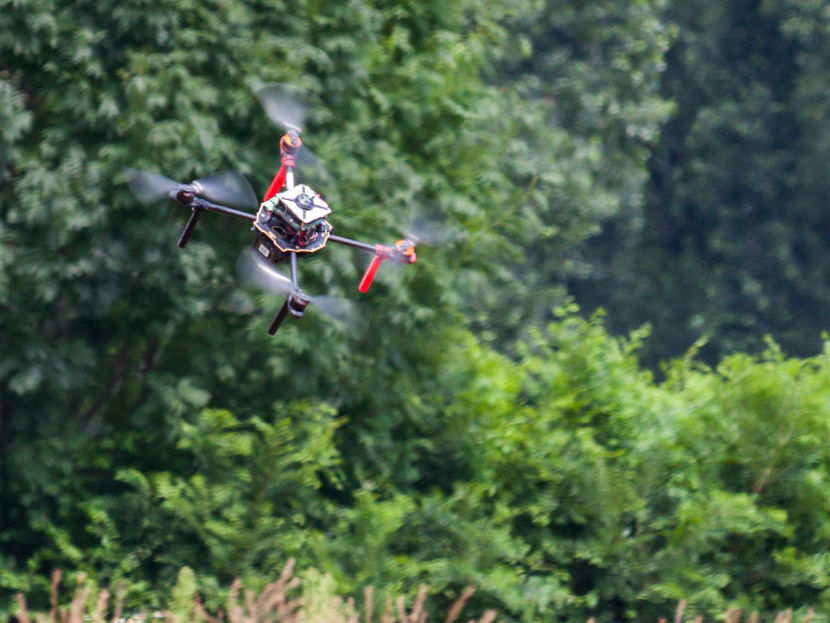
\includegraphics[width=1.0\textwidth]{./fig/drona.jpg}
  \begin{itemize}
    \item UAV control
    \item State estimation
    \item Trajectory tracking
    \item UAV deployment
  \end{itemize}
\end{block}

\column{0.31\textwidth}

\begin{block}{Remote sensing by UAVs}
  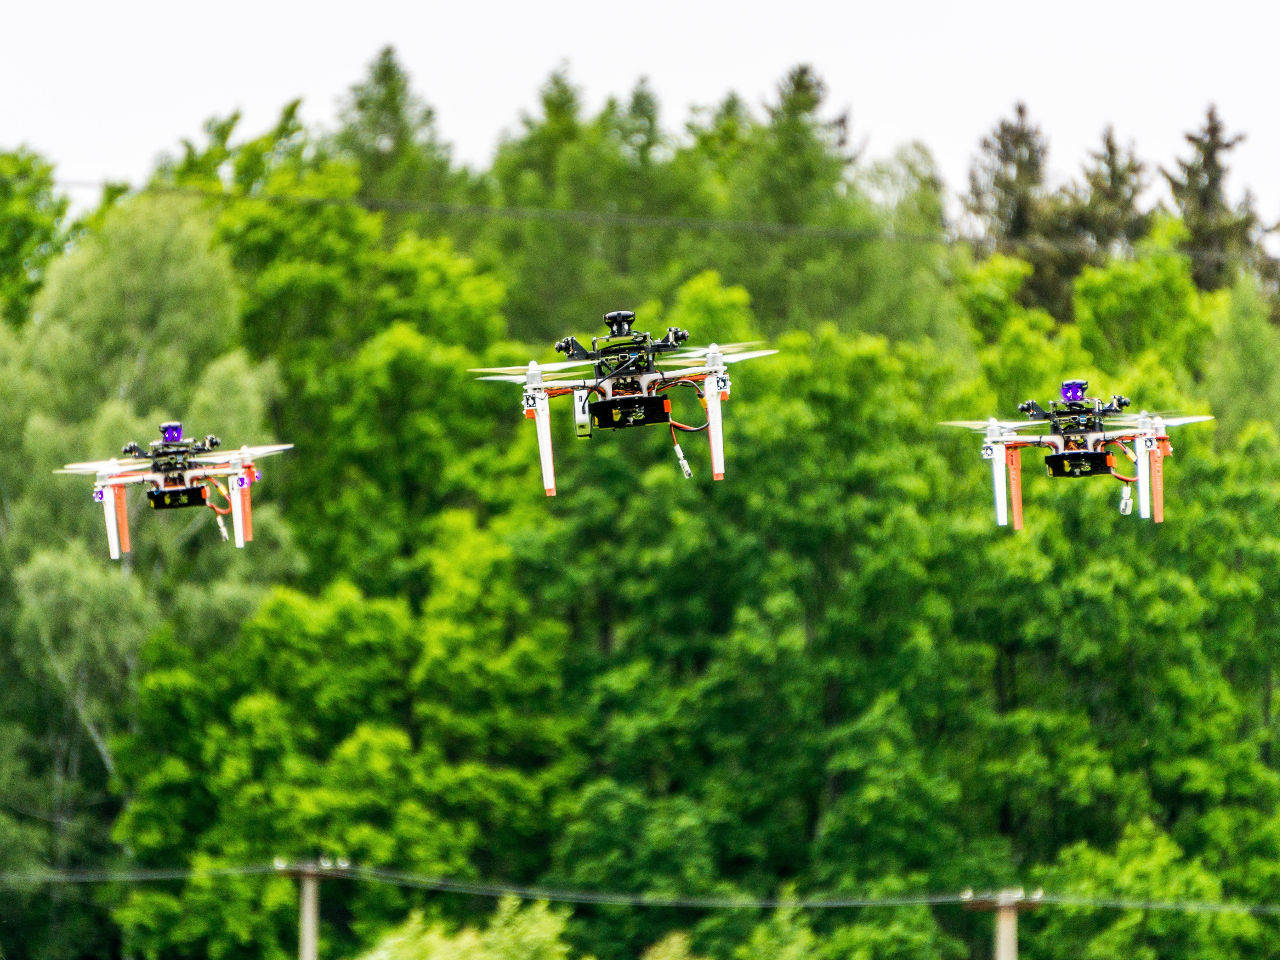
\includegraphics[width=1.0\textwidth]{./fig/photos/swarm_2_1-5.jpg}
  \begin{itemize}
    \item Object estimation
    \item Object manipulation
    \item Precise landing
    \item UAV Swarming
  \end{itemize}
\end{block}

\column{0.31\textwidth}

\begin{block}{Radiation dosimetry}
  \begin{center}
    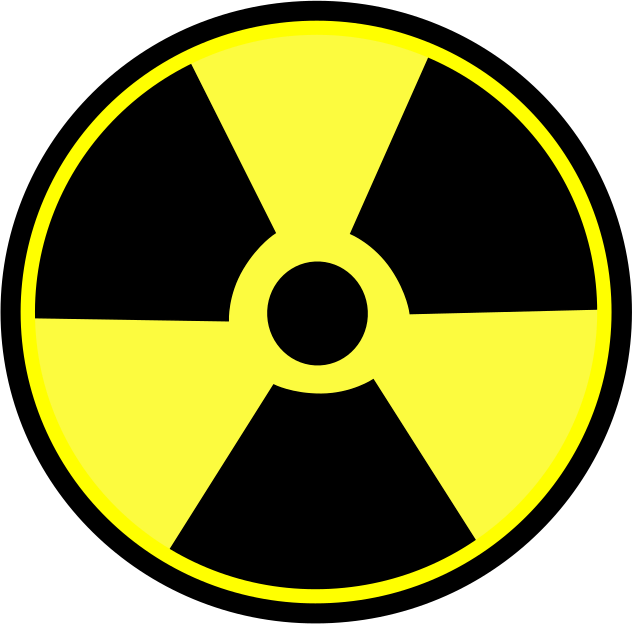
\includegraphics[width=0.70\textwidth]{./fig/photos/radioactive_sign.png}
  \end{center}
  \begin{itemize}
    \item Pixel detectors
    \item Space dosimetry
    \item Terrestrial dosimetry
    \item UAV Compton camera
  \end{itemize}
\end{block}

\end{columns}

\end{frame}

%%}

\section{Research stream 1: Multirotor-UAV system for research and real-world deployment}

\begin{frame}
  \frametitle{Outline}
  \tableofcontents[currentsection]
\end{frame}

%%{ Multirotor UAV system for research

%%{ Motivation

\begin{frame}
\frametitle{Multirotor UAV system for research}

  \begin{block}{Motivation (2013 -- 2016)}
    \begin{itemize}
      \item research validation in real-world experiments \cite{spurny2016complex, saska2016formations, chudoba2016exploration, saska2017system, saska2017documentation, saska2013adhoc, chudoba2014localization}
      \item Desired: experimenting outside of laboratory conditions, without a MoCap system
    \end{itemize}
  \end{block}

  \begin{columns}[c]

  \column{0.385\textwidth} % Left column and width

  \begin{block}{Embedded MPC \cite{baca2016embedded}}
    \centering
    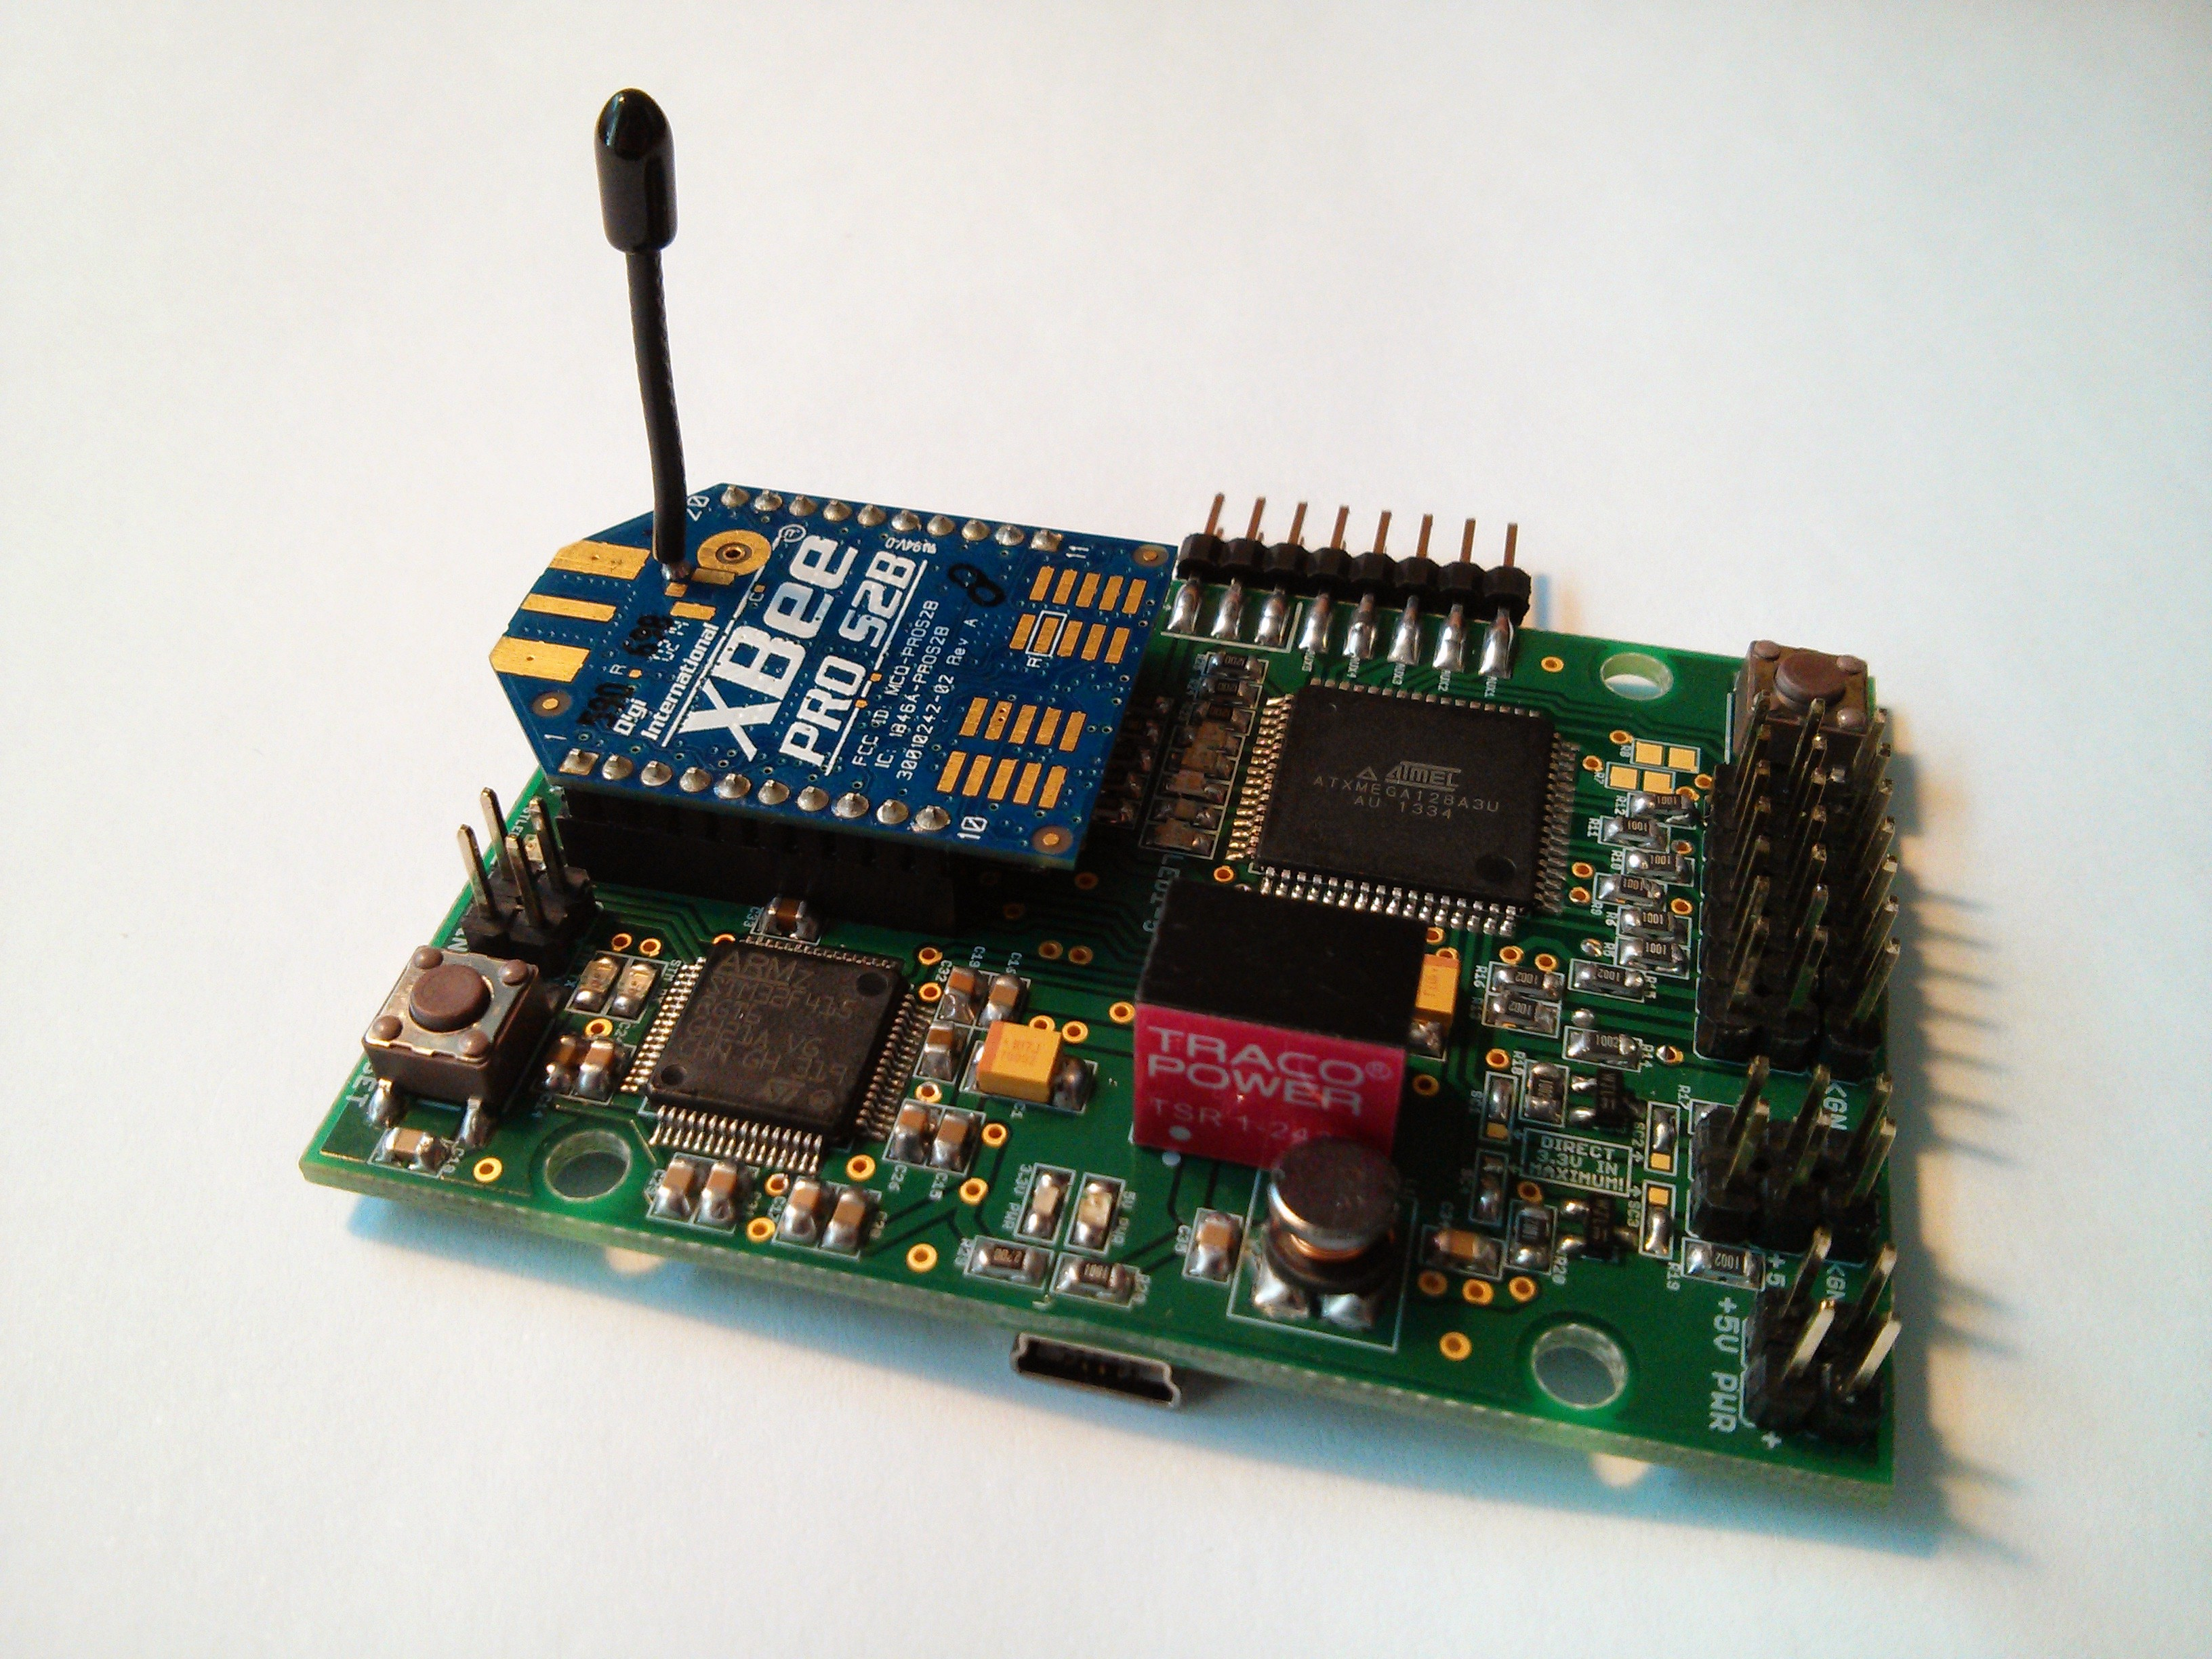
\includegraphics[width=1.0\textwidth]{./fig/photos/multirotor_control_board.jpg}
  \end{block}

  \column{0.57\textwidth} % Right column and width

  \begin{block}{Multi-UAV formations \cite{spurny2016complex}}
    \centering
    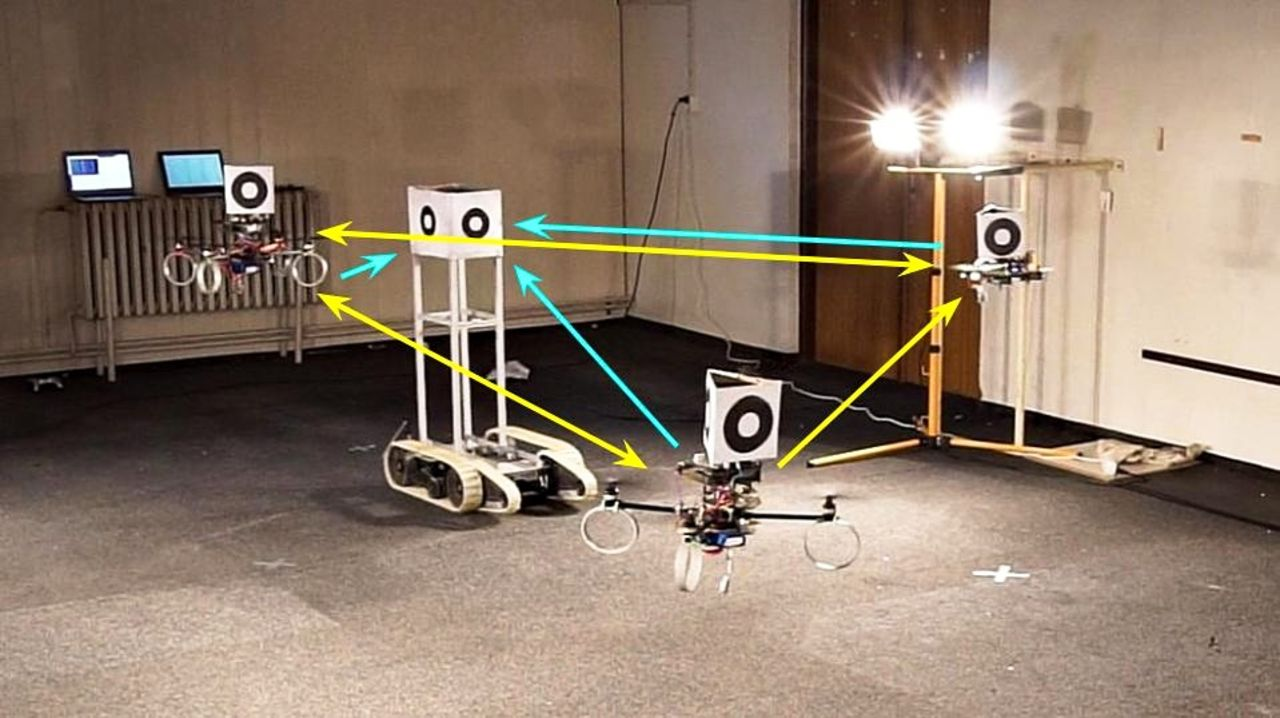
\includegraphics[width=0.9\textwidth]{./fig/photos/mav_rfid.jpg}
  \end{block}

  \end{columns}

\end{frame}

%%}

%%{ System diagram

\begin{frame}

\frametitle{The MRS UAV System}

  \begin{block}{MRS UAV System block diagram}
    \begin{figure}
      \begin{adjustbox}{max totalsize={1.0\textwidth}{.65\textheight}, center}
        \only<1>{\pgfdeclarelayer{foreground}
\pgfsetlayers{background,main,foreground}

\tikzset{radiation/.style={{decorate,decoration={expanding waves,angle=90,segment length=4pt}}}}

\begin{tikzpicture}[->,>=stealth', node distance=3.0cm]

  \node[state, shift = {(0.0, 0.0)}] (user_software) {
      \begin{tabular}{c}
        \small Mission \\
        \small planner
      \end{tabular}
    };

  \node[state, right of = user_software, shift = {(0.6, 0.0)}] (collision_avoidance) {
      \begin{tabular}{c}
        \small Collision \\
        \small avoidance
      \end{tabular}
    };

  \node[state, right of = collision_avoidance, shift = {(0, -0)}] (mpc_tracker) {
      \begin{tabular}{c}
        \small MPC \\
        \small tracker
      \end{tabular}
    };

  \node[state, right of = mpc_tracker, shift = {(0, -0)}] (so3_controller) {
      \begin{tabular}{c}
        \small SO(3) \\
        \small controller
      \end{tabular}
    };

  \node[state, right of = so3_controller, shift = {(0.2, -0)}] (pixhawk) {
      \begin{tabular}{c}
        \small Attitude \\
        \small controller
      \end{tabular}
    };

  \node[state, right of = pixhawk, shift = {(0, -0)}] (uav_plant) {
      \begin{tabular}{c}
        \small UAV \\
        \small plant
      \end{tabular}
    };

  \node[state, below of = so3_controller, shift = {(0, 0.5)}] (state_observer) {
      \begin{tabular}{c}
        \small State \\
        \small observer
      \end{tabular}
    };

    \path[->] ($(user_software.east) + (0.0, 0)$) edge [] node[above, midway, shift = {(0.0, 0.05)}] {  
      \begin{tabular}{c}
        \small desired trajectory\\
        \small $\mathbf{r}_D, \phi_D$\\
        \small \textit{on demand}
    \end{tabular}} ($(collision_avoidance.west) + (0.0, 0.00)$);

    \path[->] ($(collision_avoidance.east) + (0.0, 0)$) edge [] node[above, midway, shift = {(0.0, 0.05)}] {  
      \begin{tabular}{c}
        \small reshaped trajectory\\
        \small $\mathbf{r}_R, \phi_R$\\
        \small \textit{100 Hz}
    \end{tabular}} ($(mpc_tracker.west) + (0.0, 0.00)$);

    \path[->] ($(mpc_tracker.east) + (0.0, 0)$) edge [] node[above, midway, shift = {(0.0, 0.05)}] {  
      \begin{tabular}{c}
        % \small $\textbf{x}_D, \dot{\textbf{x}}_D, \ddot{\textbf{x}}_D$ \\
        % \small $\phi_{D}, \dot{\phi}_D, \ddot{\phi}_D$\\
        $\textbf{x}_D$\\
        \small \textit{100 Hz}
    \end{tabular}} ($(so3_controller.west) + (0.0, 0.00)$);

    \path[->] ($(so3_controller.east) + (0.0, 0)$) edge [] node[above, midway, shift = {(0.0, 0.05)}] {  
      \begin{tabular}{c}
        \small $\textbf{R}\left(\phi_D, \theta_D, \psi_D\right)$ \\
        \small $T_D$ \\
        \small \textit{100 Hz}
    \end{tabular}} ($(pixhawk.west) + (0.0, 0.00)$);

    \path[->] ($(pixhawk.east) + (0.0, 0)$) edge [] node[above, midway, shift = {(0.0, 0.05)}] {  
      \begin{tabular}{c}
        \small motor \\
        \small control \\
        \small \textit{$\approx1$ kHz}
    \end{tabular}} ($(uav_plant.west) + (0.0, 0.00)$);

    \pgfmathsetmacro{\offsetA}{-1.5}
    \coordinate (under_mpc) at ($(mpc_tracker.south) + (0.0, \offsetA)$);
    \coordinate (under_avoidance) at ($(collision_avoidance.south) + (0.0, \offsetA)$);
    \path[-] ($(mpc_tracker.south) + (0.0, 0)$) edge [] (under_mpc) -- (under_mpc) edge [] (under_avoidance) edge [] node[above, midway, shift = {(0.0, 0.0)}] {  
      \begin{tabular}{c}
        \small predicted \\
        \small trajectory \\
        \small \textit{2 Hz}
    \end{tabular}} (under_avoidance) -- (under_avoidance) edge [->] ($(collision_avoidance.south) + (0.0, 0.0)$);
    \pgfmathsetmacro{\offsetB}{-0.45}
    \path[->] ($(collision_avoidance.south)+(+\offsetB, -3.5)$) edge [dashed] node[left, near start, shift = {(0.2, -0.3)}] {  
      \begin{tabular}{c}
        \small \corrected {predicted} \\
        \small \corrected {trajectory} \\
        \small \corrected {of other UAVs} \\
        \small \corrected {\textit{2 Hz}}
    \end{tabular}} ($(collision_avoidance.south)+(+\offsetB, 0)$);

    \draw[-, radiation, decoration={angle=45}] ($(collision_avoidance.south) + (\offsetB+0.14, -3.2)$) -- +(0:0.5);

    \pgfmathsetmacro{\offsetC}{0.0}
    \path[<-] ($(mpc_tracker.south)+(+\offsetC, -3.5)$) edge [dashed] node[left, near start, shift = {(0.2, -0.3)}] {  
      \begin{tabular}{c}
        \small predicted \\ 
        \small trajectory \\
        \small \textit{2 Hz}
    \end{tabular}} ($(mpc_tracker.south)+(+\offsetC, 0)$);

    \draw[-, radiation, decoration={angle=45}] ($(mpc_tracker.south) + (0.15, -3.2)$) -- +(0:0.5);
    % \draw[-, radiation, decoration={angle=45}] ($(mpc_tracker.south) + (+0.50, -3.5)$) -- +(90:0.5);

    \path[-] ($(state_observer.west)+(0, 0)$) edge [dotted] node[above, near end, shift = {(-1.2, 0.0)}] {  
      \begin{tabular}{c}
        \small UAV state \\
        \small estimate \\
        \small \textit{100 Hz}
    \end{tabular}} ($(user_software.south |- state_observer.west)$) -- ($(user_software.south |- state_observer.west)$) edge [->,dotted] ($(user_software.south)+(0, 0)$);

    \path[->] ($(state_observer.north)+(0, 0)$) edge [dotted] ($(so3_controller.south)$);

    \path[-] ($(pixhawk.south)+(0, 0)$) edge [dotted] ($(pixhawk.south |- state_observer.east)$);

    \path[-] ($(uav_plant.south)+(0, 0)$) edge [dotted] ($(uav_plant.south |- state_observer.east)$) -- ($(uav_plant.south |- state_observer.east)$) edge [->, dotted] node[below, near start, shift = {(-0.3, 0.0)}] {  
      \begin{tabular}{c}
        \small onboard sensor data \\
        \small \textit{$\approx100$ Hz}
    \end{tabular}}($(state_observer.east)$);

  \end{tikzpicture}
}
        \only<2>{\pgfdeclarelayer{foreground}
\pgfsetlayers{background,main,foreground}

\tikzset{radiation/.style={{decorate,decoration={expanding waves,angle=90,segment length=4pt}}}}

\begin{tikzpicture}[->,>=stealth', node distance=3.0cm,scale=1.0, every node/.style={scale=1.0}]

  %%{ nodes

  \node[state, shift = {(0.0, 0.0)}] (navigation) {
      \begin{tabular}{c}
        \footnotesize Mission \&\\
        \footnotesize navigation
      \end{tabular}
    };

  % \node[state, left of = navigation, shift = {(0.5, 0.0)}] (nimbro) {
  %     \begin{tabular}{c}
  %       \footnotesize Nimbro \\
  %       \footnotesize Network
  %     \end{tabular}
  %   };

  \node[state, right of = navigation, shift = {(0.7, 0)}] (tracker) {
      \begin{tabular}{c}
        \footnotesize Reference \\
        \footnotesize tracker
      \end{tabular}
    };

  \node[state_focus, right of = tracker, shift = {(0.1, 0)}] (controller) {
      \begin{tabular}{c}
        \footnotesize Reference \\
        \footnotesize controller
      \end{tabular}
    };

  \node[state, right of = controller, shift = {(0.8, -0)}] (attitude) {
      \begin{tabular}{c}
        \footnotesize Attitude rate\\
        \footnotesize controller
      \end{tabular}
    };

  \node[smallstate, below of = attitude, shift = {(-0.6, 2.05)}] (imu) {
      \footnotesize IMU
    };

  \node[state, right of = attitude, shift = {(0.7, -0)}] (actuators) {
      \begin{tabular}{c}
        \footnotesize UAV \\
        \footnotesize actuators
      \end{tabular}
    };

  \node[state, right of = actuators, shift = {(-0.8, -0)}] (sensors) {
      \begin{tabular}{c}
        \footnotesize Onboard \\
        \footnotesize sensors
      \end{tabular}
    };

  \node[state, below of = attitude, shift = {(0, 0.9)}] (estimator) {
      \begin{tabular}{c}
        \footnotesize State \\
        \footnotesize estimator
      \end{tabular}
    };

  \node[state, right of = estimator, shift = {(0.8, 0.0)}] (localization) {
      \begin{tabular}{c}
        \footnotesize Odometry \& \\
        \footnotesize localization
      \end{tabular}
    };

  %%}

  %%{ paths

  \path[->] ($(navigation.east) + (0.0, 0)$) edge [] node[above, midway, shift = {(0.0, 0.05)}] {
      \begin{tabular}{c}
        \footnotesize desired reference\\
        \footnotesize $\mathbf{r}_d, \eta_d$\\
        \footnotesize \textit{on demand}
    \end{tabular}} ($(tracker.west) + (0.0, 0.00)$);

  % \path[->] ($(nimbro.east) + (0.0, 0)$) edge [] node[above, midway, shift = {(0.0, 0.05)}] {
  %     \begin{tabular}{c}
  %   \end{tabular}} ($(navigation.west) + (0.0, 0.00)$);

  \path[->] ($(tracker.east) + (0.0, 0)$) edge [] node[above, midway, shift = {(0.0, 0.05)}] {
      \begin{tabular}{c}
        \footnotesize full-state reference\\
        \footnotesize $\bm{\chi}_d$\\
        \footnotesize \SI{100}{\hertz}
    \end{tabular}} ($(controller.west) + (0.0, 0.00)$);

  \path[->] ($(tracker.south |- estimator.west) + (0.0, 0.0)$) edge [dotted] node[left, midway, shift = {(0.2, 0.00)}] {
      \begin{tabular}{r}
        \scriptsize initialization\\[-0.5em]
        \scriptsize only
    \end{tabular}} ($(tracker.south) + (0.0, 0.00)$);

  \path[->] ($(controller.east) + (0.0, 0)$) edge [] node[above, midway, shift = {(-0.2, 0.05)}] {
      \begin{tabular}{c}
        \footnotesize $\bm{\omega}_d$\\
        \footnotesize $T_d$ \\
        \footnotesize \SI{100}{\hertz}
    \end{tabular}} ($(attitude.west) + (0.0, 0.00)$);

  \draw[-] ($(controller.south)+(0.25,0)$) -- ($(controller.south |- estimator.west) + (0.25, 0.25)$) edge [->] node[above, near start, shift = {(-0.2, 0.05)}] {
      \begin{tabular}{c}
        \footnotesize $\mathbf{a}_d$
    \end{tabular}} ($(estimator.west) + (0, 0.25)$);

  \path[->] ($(attitude.east) + (0.0, 0)$) edge [] node[above, midway, shift = {(0.1, 0.05)}] {
      \begin{tabular}{c}
        \footnotesize $\bm{\tau}_d$ \\
        \footnotesize $\approx$\SI{1}{\kilo\hertz}
    \end{tabular}} ($(actuators.west) + (0.0, 0.00)$);

  \path[-] ($(estimator.west)+(0, 0)$) edge [] node[above, near start, shift = {(-1.0, 0.0)}] {
      \begin{tabular}{c}
        \footnotesize $\mathbf{x}$, $\mathbf{R}$, $\bm{\omega}$\\
        \footnotesize \SI{100}{\hertz}
    \end{tabular}} ($(navigation.south |- estimator.west)$) -- ($(navigation.south |- estimator.west)$) edge [->,] ($(navigation.south)+(0, 0)$);

  % \path[-] ($(estimator.west)+(0, 0)$) edge [] node[above, near start, shift = {(-1.0, 0.0)}] {
  %     \begin{tabular}{c}
  %   \end{tabular}} ($(nimbro.south |- estimator.west)$) -- ($(nimbro.south |- estimator.west)$) edge [->,] ($(nimbro.south)+(0, 0)$);

  \path[->] ($(controller.south |- estimator.west)+(0, 0)$) edge [] ($(controller.south)$);

  \draw[-] ($(imu.east) + (0.0, 0.0)$) -- ($(estimator.north |- imu.east) + (0.3, 0)$) edge [->] node[right, midway, shift = {(-0.2, 0.3)}] {
      \begin{tabular}{c}
        \footnotesize $\mathbf{R}$, $\bm{\omega}$
    \end{tabular}} ($(estimator.north) + (0.3, 0.0)$);

  \draw[-] ($(sensors.south)+(0, 0)$) -- ($(sensors.south |- localization.east)$) edge [->] ($(localization.east)$);
  \draw[-] ($(sensors.south)+(0.1, 0)$) -- ($(sensors.south |- localization.east) + (0.1, -0.1)$) edge [->] ($(localization.east) + (0.0, -0.1)$);
  \draw[-] ($(sensors.south)+(-0.1, 0)$) -- ($(sensors.south |- localization.east) + (-0.1, 0.1)$) edge [->]  ($(localization.east) + (0.0, 0.1)$);

  \draw[->] ($(localization.west)+(0, 0)$) -- ($(estimator.east)$);
  \draw[->] ($(localization.west)+(0, 0.1)$) -- ($(estimator.east) + (0, 0.1)$);
  \draw[->] ($(localization.west)+(0, -0.1)$) -- ($(estimator.east) + (0, -0.1)$);

  %%}

    % \draw[-, radiation, decoration={angle=45}] ($(nimbro.west) + (0.0, -0.0)$) -- +(0:-0.5);

  %%{ backgrounds

  \begin{pgfonlayer}{background}
    \path (attitude.west |- attitude.north)+(-0.45,0.8) node (a) {};
    \path (imu.south -| sensors.east)+(+0.25,-0.20) node (b) {};
    \path[rounded corners, draw=black!70, densely dotted]
      (a) rectangle (b);
  \end{pgfonlayer}
  \node [rectangle, above of=actuators, shift={(-0.6,0.55)}, node distance=1.7em] (autopilot) {\footnotesize UAV plant};

  \begin{pgfonlayer}{background}
    \path (attitude.west |- attitude.north)+(-0.25,0.47) node (a) {};
    \path (imu.south -| attitude.east)+(+0.25,-0.10) node (b) {};
    \path[rounded corners, draw=black!70, densely dotted]
      (a) rectangle (b);
  \end{pgfonlayer}
  \node [rectangle, above of=attitude, shift={(0,0.2)}, node distance=1.7em] (autopilot) {\footnotesize Embedded autopilot};

  %%}

\end{tikzpicture}
}
      \end{adjustbox}
    \end{figure}
  \end{block}

  \fullciteinbox{baca2021mrs}{}

\end{frame}

%%}

%%{ Controller

\begin{frame}
\frametitle{Reference controller}



\end{frame}

%%}

%%{ Estimator

\begin{frame}

\frametitle{The MRS UAV System}

  \begin{block}{MRS UAV System block diagram}
    \begin{figure}
      \begin{adjustbox}{max totalsize={1.0\textwidth}{.65\textheight}, center}
        \pgfdeclarelayer{foreground}
\pgfsetlayers{background,main,foreground}

\tikzset{radiation/.style={{decorate,decoration={expanding waves,angle=90,segment length=4pt}}}}

\begin{tikzpicture}[->,>=stealth', node distance=3.0cm,scale=1.0, every node/.style={scale=1.0}]

  %%{ nodes

  \node[state, shift = {(0.0, 0.0)}] (navigation) {
      \begin{tabular}{c}
        \footnotesize Mission \&\\
        \footnotesize navigation
      \end{tabular}
    };

  % \node[state, left of = navigation, shift = {(0.5, 0.0)}] (nimbro) {
  %     \begin{tabular}{c}
  %       \footnotesize Nimbro \\
  %       \footnotesize Network
  %     \end{tabular}
  %   };

  \node[state, right of = navigation, shift = {(0.7, 0)}] (tracker) {
      \begin{tabular}{c}
        \footnotesize Reference \\
        \footnotesize tracker
      \end{tabular}
    };

  \node[state, right of = tracker, shift = {(0.1, 0)}] (controller) {
      \begin{tabular}{c}
        \footnotesize Reference \\
        \footnotesize controller
      \end{tabular}
    };

  \node[state, right of = controller, shift = {(0.8, -0)}] (attitude) {
      \begin{tabular}{c}
        \footnotesize Attitude rate\\
        \footnotesize controller
      \end{tabular}
    };

  \node[smallstate, below of = attitude, shift = {(-0.6, 2.05)}] (imu) {
      \footnotesize IMU
    };

  \node[state, right of = attitude, shift = {(0.7, -0)}] (actuators) {
      \begin{tabular}{c}
        \footnotesize UAV \\
        \footnotesize actuators
      \end{tabular}
    };

  \node[state, right of = actuators, shift = {(-0.8, -0)}] (sensors) {
      \begin{tabular}{c}
        \footnotesize Onboard \\
        \footnotesize sensors
      \end{tabular}
    };

  \node[state_focus, below of = attitude, shift = {(0, 0.9)}] (estimator) {
      \begin{tabular}{c}
        \footnotesize State \\
        \footnotesize estimator
      \end{tabular}
    };

  \node[state, right of = estimator, shift = {(0.8, 0.0)}] (localization) {
      \begin{tabular}{c}
        \footnotesize Odometry \& \\
        \footnotesize localization
      \end{tabular}
    };

  %%}

  %%{ paths

  \path[->] ($(navigation.east) + (0.0, 0)$) edge [] node[above, midway, shift = {(0.0, 0.05)}] {
      \begin{tabular}{c}
        \footnotesize desired reference\\
        \footnotesize $\mathbf{r}_d, \eta_d$\\
        \footnotesize \textit{on demand}
    \end{tabular}} ($(tracker.west) + (0.0, 0.00)$);

  % \path[->] ($(nimbro.east) + (0.0, 0)$) edge [] node[above, midway, shift = {(0.0, 0.05)}] {
  %     \begin{tabular}{c}
  %   \end{tabular}} ($(navigation.west) + (0.0, 0.00)$);

  \path[->] ($(tracker.east) + (0.0, 0)$) edge [] node[above, midway, shift = {(0.0, 0.05)}] {
      \begin{tabular}{c}
        \footnotesize full-state reference\\
        \footnotesize $\bm{\chi}_d$\\
        \footnotesize \SI{100}{\hertz}
    \end{tabular}} ($(controller.west) + (0.0, 0.00)$);

  \path[->] ($(tracker.south |- estimator.west) + (0.0, 0.0)$) edge [dotted] node[left, midway, shift = {(0.2, 0.00)}] {
      \begin{tabular}{r}
        \scriptsize initialization\\[-0.5em]
        \scriptsize only
    \end{tabular}} ($(tracker.south) + (0.0, 0.00)$);

  \path[->] ($(controller.east) + (0.0, 0)$) edge [] node[above, midway, shift = {(-0.2, 0.05)}] {
      \begin{tabular}{c}
        \footnotesize $\bm{\omega}_d$\\
        \footnotesize $T_d$ \\
        \footnotesize \SI{100}{\hertz}
    \end{tabular}} ($(attitude.west) + (0.0, 0.00)$);

  \draw[-] ($(controller.south)+(0.25,0)$) -- ($(controller.south |- estimator.west) + (0.25, 0.25)$) edge [->] node[above, near start, shift = {(-0.2, 0.05)}] {
      \begin{tabular}{c}
        \footnotesize $\mathbf{a}_d$
    \end{tabular}} ($(estimator.west) + (0, 0.25)$);

  \path[->] ($(attitude.east) + (0.0, 0)$) edge [] node[above, midway, shift = {(0.1, 0.05)}] {
      \begin{tabular}{c}
        \footnotesize $\bm{\tau}_d$ \\
        \footnotesize $\approx$\SI{1}{\kilo\hertz}
    \end{tabular}} ($(actuators.west) + (0.0, 0.00)$);

  \path[-] ($(estimator.west)+(0, 0)$) edge [] node[above, near start, shift = {(-1.0, 0.0)}] {
      \begin{tabular}{c}
        \footnotesize $\mathbf{x}$, $\mathbf{R}$, $\bm{\omega}$\\
        \footnotesize \SI{100}{\hertz}
    \end{tabular}} ($(navigation.south |- estimator.west)$) -- ($(navigation.south |- estimator.west)$) edge [->,] ($(navigation.south)+(0, 0)$);

  % \path[-] ($(estimator.west)+(0, 0)$) edge [] node[above, near start, shift = {(-1.0, 0.0)}] {
  %     \begin{tabular}{c}
  %   \end{tabular}} ($(nimbro.south |- estimator.west)$) -- ($(nimbro.south |- estimator.west)$) edge [->,] ($(nimbro.south)+(0, 0)$);

  \path[->] ($(controller.south |- estimator.west)+(0, 0)$) edge [] ($(controller.south)$);

  \draw[-] ($(imu.east) + (0.0, 0.0)$) -- ($(estimator.north |- imu.east) + (0.3, 0)$) edge [->] node[right, midway, shift = {(-0.2, 0.3)}] {
      \begin{tabular}{c}
        \footnotesize $\mathbf{R}$, $\bm{\omega}$
    \end{tabular}} ($(estimator.north) + (0.3, 0.0)$);

  \draw[-] ($(sensors.south)+(0, 0)$) -- ($(sensors.south |- localization.east)$) edge [->] ($(localization.east)$);
  \draw[-] ($(sensors.south)+(0.1, 0)$) -- ($(sensors.south |- localization.east) + (0.1, -0.1)$) edge [->] ($(localization.east) + (0.0, -0.1)$);
  \draw[-] ($(sensors.south)+(-0.1, 0)$) -- ($(sensors.south |- localization.east) + (-0.1, 0.1)$) edge [->]  ($(localization.east) + (0.0, 0.1)$);

  \draw[->] ($(localization.west)+(0, 0)$) -- ($(estimator.east)$);
  \draw[->] ($(localization.west)+(0, 0.1)$) -- ($(estimator.east) + (0, 0.1)$);
  \draw[->] ($(localization.west)+(0, -0.1)$) -- ($(estimator.east) + (0, -0.1)$);

  %%}

    % \draw[-, radiation, decoration={angle=45}] ($(nimbro.west) + (0.0, -0.0)$) -- +(0:-0.5);

  %%{ backgrounds

  \begin{pgfonlayer}{background}
    \path (attitude.west |- attitude.north)+(-0.45,0.8) node (a) {};
    \path (imu.south -| sensors.east)+(+0.25,-0.20) node (b) {};
    \path[rounded corners, draw=black!70, densely dotted]
      (a) rectangle (b);
  \end{pgfonlayer}
  \node [rectangle, above of=actuators, shift={(-0.6,0.55)}, node distance=1.7em] (autopilot) {\footnotesize UAV plant};

  \begin{pgfonlayer}{background}
    \path (attitude.west |- attitude.north)+(-0.25,0.47) node (a) {};
    \path (imu.south -| attitude.east)+(+0.25,-0.10) node (b) {};
    \path[rounded corners, draw=black!70, densely dotted]
      (a) rectangle (b);
  \end{pgfonlayer}
  \node [rectangle, above of=attitude, shift={(0,0.2)}, node distance=1.7em] (autopilot) {\footnotesize Embedded autopilot};

  %%}

\end{tikzpicture}

      \end{adjustbox}
    \end{figure}
  \end{block}

  \fullciteinbox{baca2021mrs}{}

\end{frame}

\begin{frame}

\frametitle{The MRS UAV System}

  \begin{columns}[c]

  \column{0.55\textwidth} % Left column and width

  \begin{block}{Bank of filters}

    \begin{figure}
      \begin{adjustbox}{max totalsize={1.0\textwidth}{.65\textheight}, center}
        \usetikzlibrary{shapes.geometric,backgrounds,calc,arrows}
\pgfdeclarelayer{background}
\pgfdeclarelayer{foreground}
\pgfsetlayers{background,main,foreground}

\tikzset{radiation/.style={{decorate,decoration={expanding waves,angle=90,segment length=4pt}}}}

\begin{tikzpicture}[->,>=stealth', node distance=3.0cm]

  %%{ filters

  \def\filtx{10pt}
  \def\dotoff{1.5}
  % \node[state, shift = {(0.0, 0.0)}] (preprocess) {
  %     \begin{tabular}{c}
  %       \small Preprocess
  %     \end{tabular}
  %   };

  \node[state, shift = {(0, -0)}] (k1) {
      \begin{tabular}{c}
        \small $K_1$
      \end{tabular}
    };

  \node[state, right of = k1, shift = {(-\filtx, -0)}] (k2) {
      \begin{tabular}{c}
        \small $K_2$
      \end{tabular}
    };

  \node[right of = k2, shift = {(-\dotoff, -0)}] (kdots) {
      \begin{tabular}{c}
        \small $\cdots$
      \end{tabular}
    };

  \node[state, right of = kdots, shift = {(-\dotoff, -0)}] (kn) {
      \begin{tabular}{c}
        \small $K_n$
      \end{tabular}
    };

  %%}

  %%{ predictions, corrections

  \def\eloffx{1.5}
  \def\eloffy{1.2}
  \def\ellx{20pt}
  \def\elly{22pt}
  \node[ellipse, minimum height=\elly, minimum width=\ellx, draw, above left of = k1, shift = {(\eloffx, -\eloffy)}] (pred1) {
      \small pred
    };

  \path[->] (k1.west) [bend left]  edge node {} (pred1);
  \path[->] (pred1) [bend left]  edge node {} ([xshift=-5pt]k1.north);

  \node[ellipse, minimum height=\elly, minimum width=\ellx,  draw, above right of = k1, shift = {(-\eloffx, -\eloffy)}] (corr1) {
    \small corr
  };

  \path[->] (k1.east) [bend right]  edge node {} (corr1);
  \path[->] (corr1) [bend right]  edge node {} ([xshift=5pt]k1.north);

  \node[ellipse, minimum height=\elly, minimum width=\ellx,  draw, above left of = k2, shift = {(\eloffx, -\eloffy)}] (pred2) {
    \small pred
  };

  \path[->] (k2.west) [bend left]  edge node {} (pred2);
  \path[->] (pred2) [bend left]  edge node {} ([xshift=-5pt]k2.north);

  \node[ellipse, minimum height=\elly, minimum width=\ellx,  draw, above right of = k2, shift = {(-\eloffx, -\eloffy)}] (corr2) {
    \small corr
  };

  \path[->] (k2.east) [bend right]  edge node {} (corr2);
  \path[->] (corr2) [bend right]  edge node {} ([xshift=5pt]k2.north);

  \node[ellipse, minimum height=\elly, minimum width=\ellx,  draw, above left of = kn, shift = {(\eloffx, -\eloffy)}] (predn) {
    \small pred
  };

  \path[->] (kn.west) [bend left]  edge node {} (predn);
  \path[->] (predn) [bend left]  edge node {} ([xshift=-5pt]kn.north);

  \node[ellipse, minimum height=\elly, minimum width=\ellx,  draw, above right of = kn, shift = {(-\eloffx, -\eloffy)}] (corrn) {
    \small corr
  };

  \path[->] (kn.east) [bend right]  edge node {} (corrn);
  \path[->] (corrn) [bend right]  edge node {} ([xshift=5pt]kn.north);

  %%}

  %%{ input
  
    \def\apredy{-2}
  
    \node[above of = pred1, shift = {(0, \apredy)}] (apred1) {
    };
  
    \node[above of = pred2, shift = {(0, \apredy)}] (apred2) {
    };
  
    \node[above of = predn, shift = {(0, \apredy)}] (apredn) {
    };
  
    \node[left of = apred1, shift = {(2, 0)}] (input) {
    };
  
  % node[above] {$\mathbf{T}_{total}$}
    \path[-] (input.center) edge node [above, shift = {(-0.3,0)}] {$\mathbf{u}$} (apred1.center);
    \path[-] (apred1.center) edge node {} (apred2.center);
    \path[-] (apred2.center) edge node {} (apredn.center);
  
    \path[->] (apred1.center) edge node {} (pred1.north);
    \path[->] (apred2.center) edge node {} (pred2.north);
    \path[->] (apredn.center) edge node {} (predn.north);
  
  %%}

  %%{ measurement
  
    \def\apredy{-2.2}
  
    \node[above of = corr1, shift = {(0, \apredy)}] (acorr1) {
    };
  
    \node[above of = corr2, shift = {(0, \apredy)}] (acorr2) {
    };
  
    \node[above of = corrn, shift = {(0, \apredy)}] (acorrn) {
    };
  
    \node[left of = acorr1, shift = {(1, 0)}] (measurement) {
    };
  
  % node[above] {$\mathbf{T}_{total}$}
    \path[-] (measurement.center) edge node [below, shift = {(-0.8,0)}] {$\mathbf{z}$} (acorr1.center);
    \path[-] (acorr1.center) edge node {} (acorr2.center);
    \path[-] (acorr2.center) edge node {} (acorrn.center);
  
    \path[->] (acorr1.center) edge node {} (corr1.north);
    \path[->] (acorr2.center) edge node {} (corr2.north);
    \path[->] (acorrn.center) edge node {} (corrn.north);
  
  %%}

  %%{ arbiter

  \def\mararb{5pt}
  \def\cs{5pt}
  \def\offcx{2}
  \def\offcy{1.5}

  \node[circle, inner sep=0pt, minimum size=\cs,  draw, below of = k2, shift = {(0,\offcy)}] (contact2) {
  };

  \node[circle, inner sep=0pt, minimum size=\cs,  draw, right of = contact2, shift = {(-\offcx, 0)}] (contactn) {
  };

  \node[circle, fill, inner sep=0pt, minimum size=\cs,  draw, left of = contact2, shift = {(\offcx, 0)}] (contact1) {
  };

  \def\pbky{10pt}
  \node[below of = k1, shift = {(0, 1.5*\offcy)}] (pbk1) {
  };


  \node[below of = kn, shift = {(0, 1.5*\offcy)}] (pbkn) {
  };

  \node[above of = contact1, shift = {(0, -1.5*\offcy)}] (pacontact1) {
  };

  \node[above of = contactn, shift = {(0, -1.5*\offcy)}] (pacontactn) {
  };

  % \node[circle, inner sep=0pt, minimum size=\cs,  draw, below of = contact2, shift = {(0,2.5)}] (contactb) {
  % };

  \node[below of = contact2, shift = {(0, 2.5)}] (contactb) {
  };

  \node[below of = contactb, shift = {(0, 2.5)}] (barbiter) {
  };

  \node[right of = barbiter, shift = {(0, 0)}] (estimate) {
  };

  \path[-] (k1.south) edge node {} (pbk1.center);
  \path[-] (pbk1.center) edge node {} (pacontact1.center);
\path[-] (pacontact1.center) edge node [below left, shift ={(-0.5,0.4)}] {$\mathbf{x}_1, \mathbf{\Sigma}_1$} (contact1.north);

\path[-] (k2.south) edge node [right, shift = {(0,0.34)}] {$\mathbf{x}_2, \mathbf{\Sigma}_2$} (contact2.north);

  \path[-] (kn.south) edge node {} (pbkn.center);
  \path[-] (pbkn.center) edge node {} (pacontactn.center);
\path[-] (pacontactn.center) edge node [below right, shift = {(0.5,0.4)}] {$\mathbf{x}_n, \mathbf{\Sigma}_n$} (contactn.north);

  \path[-] (contact1.south) edge node {} (contactb.center);
  \path[-,dotted] (contact2.south) edge node {} (contactb.center);
  \path[-,dotted] (contactn.south) edge node {} (contactb.center);

  \path[-] (contactb.center) edge node {} (barbiter.center);

  % \path[-] (kn.south) edge node {} (pbkn.center);
  % \path[-] (pbkn.center) edge node {} (pakn.center);
  % \path[-] (pakn.center) edge node {} (contactno.north);

  \node[state, inner sep = 0cm, minimum width=2.8cm, minimum height = 1cm, below of = k2, shift = {(-0, \offcy-0.25)}] (arbiter) {
    \begin{tabular}{ccccr}
      \\
      & & & & \small Arbiter
    \end{tabular}
  };

  %%}

  %%{ output
  
    \node[right of = barbiter, shift = {(0, 0)}] (output) {
    };
  
  % node[above] {$\mathbf{T}_{total}$}
    \path[->] (barbiter.center) edge node [above, shift = {(1,0)}] {$\mathbf{x}_{\ast }$} (output.center);
  
  
  %%}

\end{tikzpicture}

      \end{adjustbox}
    \end{figure}

  \end{block}

  \column{0.40\textwidth} % Right column and width

  \begin{itemize}
    \item simultaneous estimation of UAV state in multiple frames of reference
    \item automatic \& manual switching of the main estimator
    \item automatic detection of estimator failures
    \item switching of an estimator is synchronizes throughout the control pipeline
  \end{itemize}

  \end{columns}

  \fullciteinbox{petrlik2020robust}{}

\end{frame}

%%}

%%{ MPC Tracker

%% | ----------------------- MPC Tracker ---------------------- |

\begin{frame}
\frametitle{The MRS UAV System}

  \begin{block}{MRS UAV System block diagram}
    \begin{figure}
      \begin{adjustbox}{max totalsize={1.0\textwidth}{.65\textheight}, center}
        \pgfdeclarelayer{foreground}
\pgfsetlayers{background,main,foreground}

\tikzset{radiation/.style={{decorate,decoration={expanding waves,angle=90,segment length=4pt}}}}

\begin{tikzpicture}[->,>=stealth', node distance=3.0cm,scale=1.0, every node/.style={scale=1.0}]

  %%{ nodes

  \node[state, shift = {(0.0, 0.0)}] (navigation) {
      \begin{tabular}{c}
        \footnotesize Mission \&\\
        \footnotesize navigation
      \end{tabular}
    };

  % \node[state, left of = navigation, shift = {(0.5, 0.0)}] (nimbro) {
  %     \begin{tabular}{c}
  %       \footnotesize Nimbro \\
  %       \footnotesize Network
  %     \end{tabular}
  %   };

  \node[state_focus, right of = navigation, shift = {(0.7, 0)}] (tracker) {
      \begin{tabular}{c}
        \footnotesize Reference \\
        \footnotesize tracker
      \end{tabular}
    };

  \node[state, right of = tracker, shift = {(0.1, 0)}] (controller) {
      \begin{tabular}{c}
        \footnotesize Reference \\
        \footnotesize controller
      \end{tabular}
    };

  \node[state, right of = controller, shift = {(0.8, -0)}] (attitude) {
      \begin{tabular}{c}
        \footnotesize Attitude rate\\
        \footnotesize controller
      \end{tabular}
    };

  \node[smallstate, below of = attitude, shift = {(-0.6, 2.05)}] (imu) {
      \footnotesize IMU
    };

  \node[state, right of = attitude, shift = {(0.7, -0)}] (actuators) {
      \begin{tabular}{c}
        \footnotesize UAV \\
        \footnotesize actuators
      \end{tabular}
    };

  \node[state, right of = actuators, shift = {(-0.8, -0)}] (sensors) {
      \begin{tabular}{c}
        \footnotesize Onboard \\
        \footnotesize sensors
      \end{tabular}
    };

  \node[state, below of = attitude, shift = {(0, 0.9)}] (estimator) {
      \begin{tabular}{c}
        \footnotesize State \\
        \footnotesize estimator
      \end{tabular}
    };

  \node[state, right of = estimator, shift = {(0.8, 0.0)}] (localization) {
      \begin{tabular}{c}
        \footnotesize Odometry \& \\
        \footnotesize localization
      \end{tabular}
    };

  %%}

  %%{ paths

  \path[->] ($(navigation.east) + (0.0, 0)$) edge [] node[above, midway, shift = {(0.0, 0.05)}] {
      \begin{tabular}{c}
        \footnotesize desired reference\\
        \footnotesize $\mathbf{r}_d, \eta_d$\\
        \footnotesize \textit{on demand}
    \end{tabular}} ($(tracker.west) + (0.0, 0.00)$);

  % \path[->] ($(nimbro.east) + (0.0, 0)$) edge [] node[above, midway, shift = {(0.0, 0.05)}] {
  %     \begin{tabular}{c}
  %   \end{tabular}} ($(navigation.west) + (0.0, 0.00)$);

  \path[->] ($(tracker.east) + (0.0, 0)$) edge [] node[above, midway, shift = {(0.0, 0.05)}] {
      \begin{tabular}{c}
        \footnotesize full-state reference\\
        \footnotesize $\bm{\chi}_d$\\
        \footnotesize \SI{100}{\hertz}
    \end{tabular}} ($(controller.west) + (0.0, 0.00)$);

  \path[->] ($(tracker.south |- estimator.west) + (0.0, 0.0)$) edge [dotted] node[left, midway, shift = {(0.2, 0.00)}] {
      \begin{tabular}{r}
        \scriptsize initialization\\[-0.5em]
        \scriptsize only
    \end{tabular}} ($(tracker.south) + (0.0, 0.00)$);

  \path[->] ($(controller.east) + (0.0, 0)$) edge [] node[above, midway, shift = {(-0.2, 0.05)}] {
      \begin{tabular}{c}
        \footnotesize $\bm{\omega}_d$\\
        \footnotesize $T_d$ \\
        \footnotesize \SI{100}{\hertz}
    \end{tabular}} ($(attitude.west) + (0.0, 0.00)$);

  \draw[-] ($(controller.south)+(0.25,0)$) -- ($(controller.south |- estimator.west) + (0.25, 0.25)$) edge [->] node[above, near start, shift = {(-0.2, 0.05)}] {
      \begin{tabular}{c}
        \footnotesize $\mathbf{a}_d$
    \end{tabular}} ($(estimator.west) + (0, 0.25)$);

  \path[->] ($(attitude.east) + (0.0, 0)$) edge [] node[above, midway, shift = {(0.1, 0.05)}] {
      \begin{tabular}{c}
        \footnotesize $\bm{\tau}_d$ \\
        \footnotesize $\approx$\SI{1}{\kilo\hertz}
    \end{tabular}} ($(actuators.west) + (0.0, 0.00)$);

  \path[-] ($(estimator.west)+(0, 0)$) edge [] node[above, near start, shift = {(-1.0, 0.0)}] {
      \begin{tabular}{c}
        \footnotesize $\mathbf{x}$, $\mathbf{R}$, $\bm{\omega}$\\
        \footnotesize \SI{100}{\hertz}
    \end{tabular}} ($(navigation.south |- estimator.west)$) -- ($(navigation.south |- estimator.west)$) edge [->,] ($(navigation.south)+(0, 0)$);

  % \path[-] ($(estimator.west)+(0, 0)$) edge [] node[above, near start, shift = {(-1.0, 0.0)}] {
  %     \begin{tabular}{c}
  %   \end{tabular}} ($(nimbro.south |- estimator.west)$) -- ($(nimbro.south |- estimator.west)$) edge [->,] ($(nimbro.south)+(0, 0)$);

  \path[->] ($(controller.south |- estimator.west)+(0, 0)$) edge [] ($(controller.south)$);

  \draw[-] ($(imu.east) + (0.0, 0.0)$) -- ($(estimator.north |- imu.east) + (0.3, 0)$) edge [->] node[right, midway, shift = {(-0.2, 0.3)}] {
      \begin{tabular}{c}
        \footnotesize $\mathbf{R}$, $\bm{\omega}$
    \end{tabular}} ($(estimator.north) + (0.3, 0.0)$);

  \draw[-] ($(sensors.south)+(0, 0)$) -- ($(sensors.south |- localization.east)$) edge [->] ($(localization.east)$);
  \draw[-] ($(sensors.south)+(0.1, 0)$) -- ($(sensors.south |- localization.east) + (0.1, -0.1)$) edge [->] ($(localization.east) + (0.0, -0.1)$);
  \draw[-] ($(sensors.south)+(-0.1, 0)$) -- ($(sensors.south |- localization.east) + (-0.1, 0.1)$) edge [->]  ($(localization.east) + (0.0, 0.1)$);

  \draw[->] ($(localization.west)+(0, 0)$) -- ($(estimator.east)$);
  \draw[->] ($(localization.west)+(0, 0.1)$) -- ($(estimator.east) + (0, 0.1)$);
  \draw[->] ($(localization.west)+(0, -0.1)$) -- ($(estimator.east) + (0, -0.1)$);

  %%}

    % \draw[-, radiation, decoration={angle=45}] ($(nimbro.west) + (0.0, -0.0)$) -- +(0:-0.5);

  %%{ backgrounds

  \begin{pgfonlayer}{background}
    \path (attitude.west |- attitude.north)+(-0.45,0.8) node (a) {};
    \path (imu.south -| sensors.east)+(+0.25,-0.20) node (b) {};
    \path[rounded corners, draw=black!70, densely dotted]
      (a) rectangle (b);
  \end{pgfonlayer}
  \node [rectangle, above of=actuators, shift={(-0.6,0.55)}, node distance=1.7em] (autopilot) {\footnotesize UAV plant};

  \begin{pgfonlayer}{background}
    \path (attitude.west |- attitude.north)+(-0.25,0.47) node (a) {};
    \path (imu.south -| attitude.east)+(+0.25,-0.10) node (b) {};
    \path[rounded corners, draw=black!70, densely dotted]
      (a) rectangle (b);
  \end{pgfonlayer}
  \node [rectangle, above of=attitude, shift={(0,0.2)}, node distance=1.7em] (autopilot) {\footnotesize Embedded autopilot};

  %%}

\end{tikzpicture}

      \end{adjustbox}
    \end{figure}
  \end{block}

  \fullciteinbox{baca2021mrs}{}

\end{frame}

\begin{frame}
\frametitle{Model Predictive Control Tracker}

\textbf{Feedback and Feed-forward multicopter controllers benefit from a smooth and feasible control reference. A step in desired position or velocity is not a feasible reference.}

\begin{columns}[c]

\column{0.48\textwidth} % Left column and width

\begin{block}{Problem}
  \begin{itemize}
    \item real-time reference generation
    \item \SI{100}{\hertz} full state reference for controllers: $\dot{\textbf{x}}, \ddot{\textbf{x}}, \dot{\ddot{\textbf{x}}}$, $\ddot{\ddot{\textbf{x}}}$, where $\textbf{x} = \begin{pmatrix}
    r_x, r_y, r_z, \theta
    \end{pmatrix}^\intercal$ (pose and heading)
    \item UAV dynamics constraints satisfaction
    \item user input: trajectory consisting of poses sampled at regular intervals
  \end{itemize}
\end{block}

\column{0.48\textwidth} % Right column and width

\begin{block}{Solution}
  \begin{itemize}
    \item onboard real-time simulation of the linear translational UAV dynamics
    \item linear MPC (LCQP) solved at 100 Hz
    \item states of the simulated model sampled and taken as control reference
    \item \SI{8}{\second} prediction horizon used for inter-UAV collision avoidance
  \end{itemize} 
\end{block}

\end{columns}

\fullciteinbox{baca2018model}{}

\end{frame}

\begin{frame}
\frametitle{Model Predictive Control Tracker}

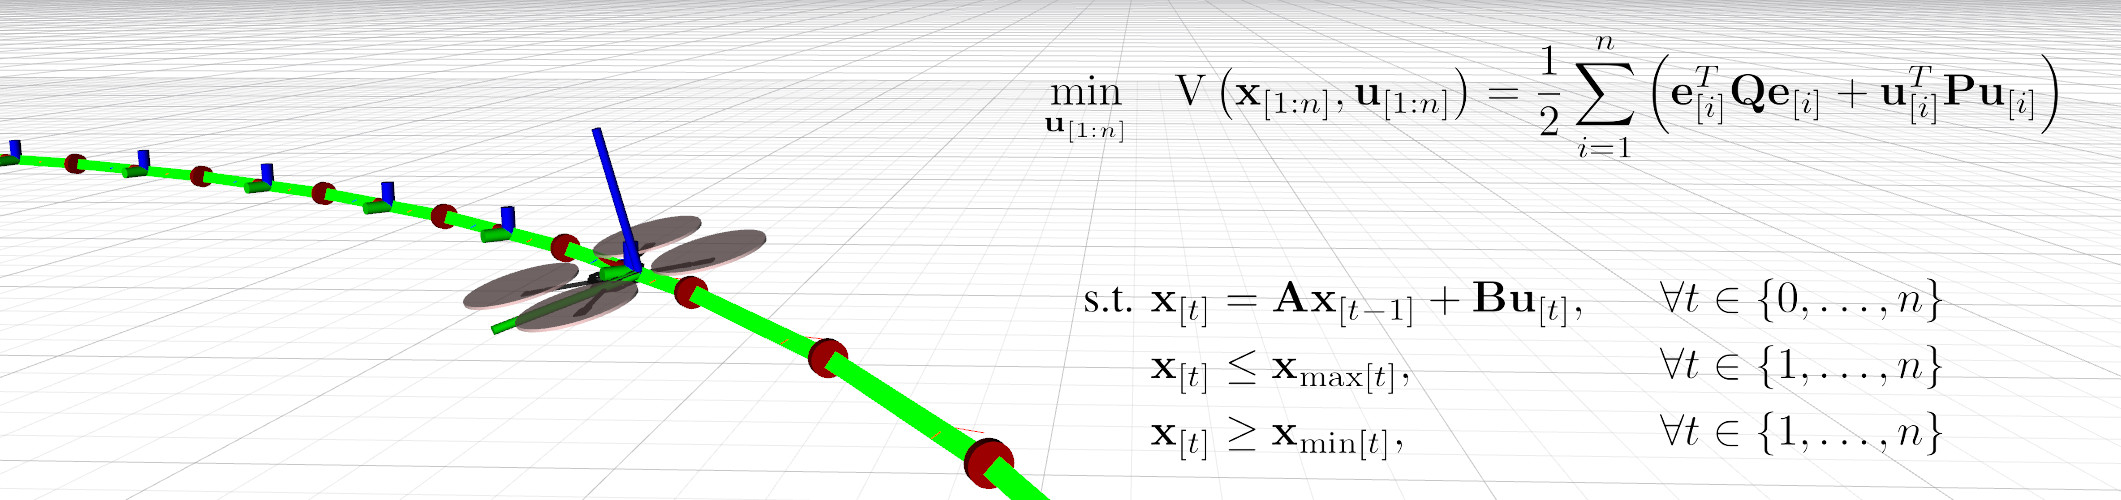
\includegraphics[width=1.0\textwidth,trim={0 0.5cm 0 1.0cm},clip]{./fig/photos/tracker.jpg}

\begin{block}{Properties}

  \vspace{-1em}

  \begin{columns}[c]

  \column{0.48\textwidth} % Left column and width

  \begin{itemize}
    \item Linear MPC is solved in real time
    \item Mutual collision avoidance prevent damage during experimentation
  \end{itemize}
  
  \column{0.48\textwidth} % Right column and width
  \begin{itemize}
    \item The LCQP can be solved reliably
    \item The tracker can handle unfeasible trajectory references from a user
  \end{itemize}
  
  \end{columns}

\end{block}

% \fullciteinbox{baca2018model}{http://github.com/ctu-mrs/mrs_uav_trackers}
\fullciteinbox{baca2018model}{}

\end{frame}

%%}

%%}

\section{Research stream 2: UAVs in remote sensing, data gathering, swarming}

\begin{frame}
  \frametitle{Outline}
  \tableofcontents[currentsection]
\end{frame}

%%{ UAVs in remote sensing, data gathering, and swarming

%%{ MBZIRC 2017 objects

\begin{frame}
\frametitle{Autonomous grasping \& delivery of objects (MBZIRC 2017)}

\begin{columns}[c]

\column{0.60\textwidth} % Left column and width

\begin{block}{Autonomous grasping and delivery of objects}
  \begin{center}
    \mymovie[autostart,loop]{
      \includegraphics[width=0.95\textwidth]{./videos/mbzirc_grasping_short_thumbnail.jpg}
    }{./videos/mbzirc_grasping_short.mp4}\\
  \end{center}
\end{block}

\column{0.35\textwidth} % Right column and width

\begin{itemize}
  \item Random initial conditions, moving objects, limited preparation time, extreme weather conditions
  \item Contribution: UAV state estimation, trajectory generation and tracking, UAV reactive collision avoidance \cite{baca2018model}, object state estimation and prediction, grasping manoeuvre
  \item Placed $1^{\mathrm{st}}$ (won \$320 000)
\end{itemize}

\end{columns}

\fullciteinbox{spurny2019cooperative}{}

\end{frame}

%%}

%%{ MBZIRC 2017 landing

\begin{frame}
\frametitle{Autonomous landing on a moving car (MBZIRC 2017)}

\begin{columns}[c]

\column{0.65\textwidth} % Left column and width

\begin{block}{Autonomous landing on a moving car}
  \begin{center}
    \mymovie[autostart,loop]{
      \includegraphics[width=0.95\textwidth]{./videos/mbzirc_landing_short_thumbnail.jpg}
    }{./videos/mbzirc_landing_short.mp4}\\
  \end{center}
\end{block}

\column{0.32\textwidth} % Right column and width

\begin{itemize}
  \item \SI{15}{\kilo\meter\per\hour} speed, random initial conditions
  \item Contribution: UAV state estimation, UAV trajectory generation and tracking, car state estimation and prediction, landing manoeuvre
  \item Fastest landing among all the teams (\SI{25}{\second})
  \item Placed $2^{\mathrm{nd}}$
\end{itemize}

\end{columns}

\fullciteinbox{baca2019autonomous}{}

\end{frame}

%%}

%%{ MBZIRC 2020 bricks

\begin{frame}
\frametitle{Autonomous wall-building by a UAVs (MBZIRC 2020)}

\begin{columns}[c]

\column{0.60\textwidth} % Left column and width

\begin{block}{Autonomous wall-building by group of 3 UAVs}
  \begin{center}
    \mymovie[autostart,loop]{
      \includegraphics[width=0.95\textwidth]{./videos/mbzirc_2020_bricks_short_thumbnail.jpg}
    }{./videos/mbzirc_2020_bricks_short.mp4}\\
  \end{center}
\end{block}

\column{0.35\textwidth} % Right column and width

\begin{itemize}
  \item Onboard detection and computation only, no RTK GPS, randomized initial conditions
  \item Contribution: UAV system, UAV control, trajectory generation, brick grasping, brick estimation, wall estimation, outlier filtering
  \item Placed $1^{\mathrm{st}}$ (won \$250 000) 
\end{itemize}

\end{columns}
\fullciteinbox{baca2020autonomous}{}

\end{frame}

%%}

%%{ MBZIRC 2020 others

\begin{frame}
\frametitle{MBZIRC 2020 --- other achievements}

\begin{columns}[c]

\column{0.48\textwidth} % Left column and width

\vspace{-1em}

\begin{block}{\small Aerial firefighting (outdoors) \cite{walter2020extinguishing, walter2021extinguishing}}
  \begin{center}
    \mymovie[autostart,loop]{
      \includegraphics[width=0.75\textwidth]{./videos/mbzirc_2020_outdoor_fires_short_thumbnail.jpg}
    }{./videos/mbzirc_2020_outdoor_fires_short.mp4}\\
  \end{center}
\end{block}

\vspace{-1em}

\begin{block}{\small Aerial static target elimination \cite{stasinchuk2021multiuav}}
  \begin{center}
    \mymovie[autostart,loop]{
      \includegraphics[width=0.75\textwidth]{./videos/mbzirc_2020_balloons_short_thumbnail.jpg}
    }{./videos/mbzirc_2020_balloons_short.mp4}\\
  \end{center}
\end{block}

\column{0.48\textwidth} % Right column and width

\vspace{-1em}

\begin{block}{\small Aerial firefighting (indoors) \cite{spurny2021autonomous}}
  \begin{center}
    \mymovie[autostart,loop]{
      \includegraphics[width=0.75\textwidth]{./videos/mbzirc_2020_indoor_fires_short_thumbnail.jpg}
    }{./videos/mbzirc_2020_indoor_fires_short.mp4}\\
  \end{center}
\end{block}

\vspace{-1em}

\begin{block}{\small Aerial moving target elimination \cite{vrba2020autonomous}}
  \begin{center}
    \mymovie[autostart,loop]{
      \includegraphics[width=0.75\textwidth]{./videos/mbzirc_2020_ball_short_thumbnail.jpg}
    }{./videos/mbzirc_2020_ball_short.mp4}\\
  \end{center}

\end{block}

\end{columns}

\end{frame}

%%}

%%{ SWARMING

\begin{frame}
\frametitle{Aerial swarming}

\begin{block}{UAV swarming and flocking}
  \begin{itemize}
    \item Distributed swarming, indoors and outdoors \cite{petracek2020bioinspired, saska2020formation, ahmad2021autonomous, dmytruk2021safe}.
    \item Contribution: UAV system, UAV control, UAV deployment
  \end{itemize}
\end{block}

\begin{columns}[c]

\column{0.48\textwidth} % Left column and width

  \begin{block}{\small Aerial swarming (GPS)}
    \begin{center}
      \mymovie[autostart,loop]{
        \includegraphics[width=0.9\textwidth]{./videos/swarm_14uavs_field_thumbnail.jpg}
      }{./videos/swarm_14uavs_field.mp4}\\
    \end{center}
  \end{block}

\column{0.48\textwidth} % Right column and width

  \begin{block}{\small Aerial swarming (GPS)}
  \begin{center}
    \mymovie[autostart,loop,start=93,stop=126]{
      \includegraphics[width=0.9\textwidth]{./videos/forest_swarm_4_uavs_rviz_thumbnail.jpg}
    }{./videos/forest_swarm_4_uavs_rviz.mp4}\\
  \end{center}
\end{block}

\end{columns}

\end{frame}

%%}

%%{ DARPA SubT

\begin{frame}
\frametitle{Aerial Search and Rescue}

\begin{block}{DARPA Subterranean (2019--2021)}
  \begin{itemize}
    \item Search for survivors in underground (mines, urban, caves) \cite{petracek2021large, kratky2021autonomous2, roucek2021system, roucek2019darpa, petrlik2020robust}.
    \item Contribution: UAV system, UAV control, trajectory tracking, trajectory generation \cite{baca2021mrs}
    \item Placed $2^{\mathrm{nd}}$ (won \$500 000 USD) in the \emph{Virtual Finals}
  \end{itemize}
\end{block}

\begin{columns}[c]

\column{0.48\textwidth} % Left column and width

  \begin{block}{Mine exploration}
    \begin{center}
      \mymovie[autostart,loop]{
        \includegraphics[width=0.9\textwidth]{./videos/darpa_finals_green_short_thumbnail.jpg}
      }{./videos/darpa_finals_green_short.mp4}\\
    \end{center}
  \end{block}

\column{0.48\textwidth} % Right column and width

  \begin{block}{Virtual cave exploration}
  \begin{center}
    \mymovie[autostart,loop]{
      \includegraphics[width=0.9\textwidth]{./videos/darpa_virtual_cave_thumbnail.jpg}
    }{./videos/darpa_virtual_cave.mp4}\\
  \end{center}
\end{block}

\end{columns}

\end{frame}

%%}

%%}

\section{Research stream 3: Ionizing radiation dosimetry and imaging}

\begin{frame}
  \frametitle{Outline}
  \tableofcontents[currentsection]
\end{frame}

%%{ Ionizing radiation dosimetry and imaging

%%{ Timepix

\begin{frame}
\frametitle{Ionizing radiation dosimetry and imaging}

  \begin{columns}[c]

  \column{0.48\textwidth} % Left column and width
  \begin{block}{Radiation pixel detectors -- Timepix}
    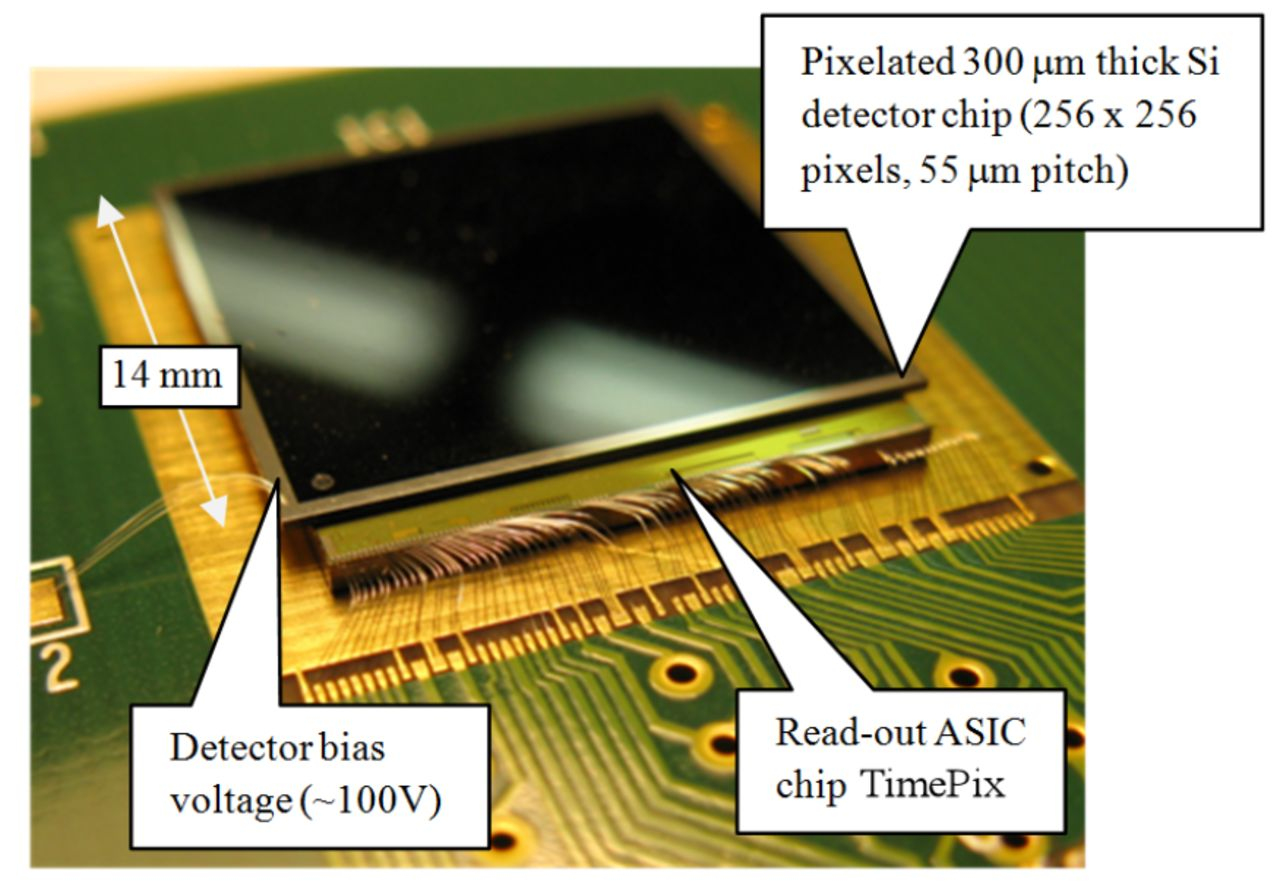
\includegraphics[width=1.0\textwidth]{./fig/timepix.jpg}
  \end{block} 

  \column{0.48\textwidth} % Right column and width
  \begin{block}{Timepix}
    \begin{itemize}
      \item 256$\times$256 px resolution
      \item frame-based acquisition
      \item event counting mode
      \item energy measurement mode
    \end{itemize}
  \end{block}

  \begin{block}{Timepix3}
    \begin{itemize}
      \item 256$\times$256 px resolution
      \item event-based acquisition
      \item event \& energy simultaneously
    \end{itemize}
  \end{block}

  \end{columns}

  \begin{block}{2013--2015}
    Work for IEAP (CTU in Prague) and Rigaku Innovative Technologies 
  \end{block}

\end{frame}

\begin{frame}
\frametitle{Timepix - Ionizing radiation dosimetry and imaging}

\begin{columns}[c]

\column{0.48\textwidth} % Right column and width

\begin{itemize}
  \item real-time recording of the interaction of an incoming particle and the sensor
  \item pattern recognition can be applied to distinguish particle types \cite{baca2018timepix}
  \item no dark-current noise
\end{itemize}

\begin{block}{Examples in the Figure}
\begin{enumerate}[label=(\alph*)]
  \item photons (gamma)
  \item electrons (beta)
  \item Helium nuclei (alpha)
  \item protons (heavy ions)
\end{enumerate}
\end{block}

\column{0.48\textwidth} % Left column and width
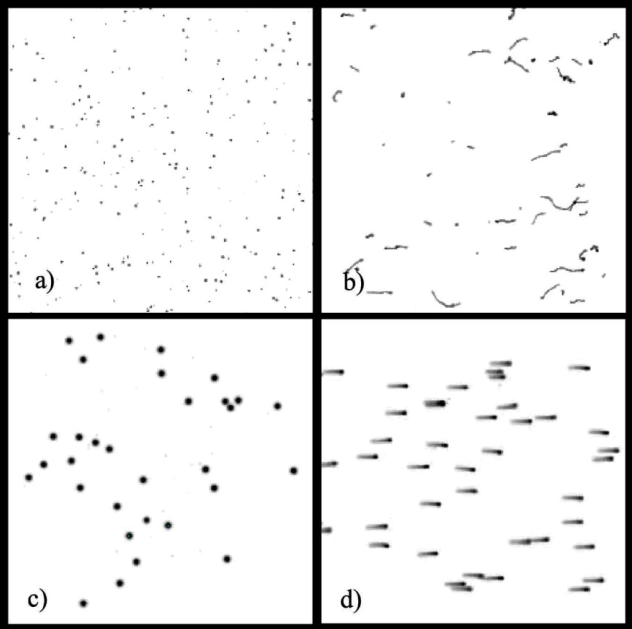
\includegraphics[width=1.0\textwidth]{./fig/particle_types_inverted.png}

\end{columns}

\end{frame}

%%}

%%{ VZLUSAT

\begin{frame}
\frametitle{VZLUSAT-1}

\begin{columns}[c]

\column{0.65\textwidth} % Left column and width

\begin{block}{VZLUSAT-1 --- The first Czech CubeSat \cite{urban2017vzlusat, baca2016miniaturized}}
  \begin{itemize}
    \item \small Custom-designed embedded Timepix board and software \cite{baca2016miniaturized}
    \item \small Onboard image processing, filtering, automated acquisition
    \item \small The longest-operating Czech(-oslovakian) sat. (2017--now)
  \end{itemize}
\end{block}

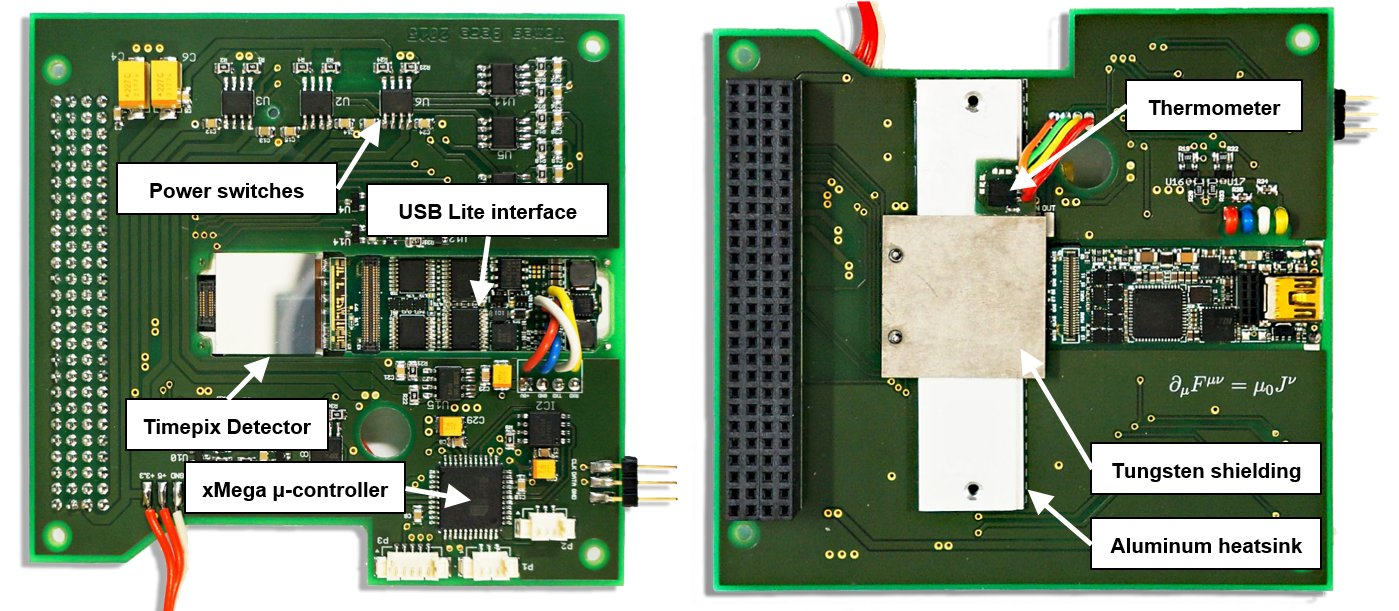
\includegraphics[width=1.0\textwidth]{./fig/photos/boards.jpg}

\column{0.3\textwidth} % Right column and width

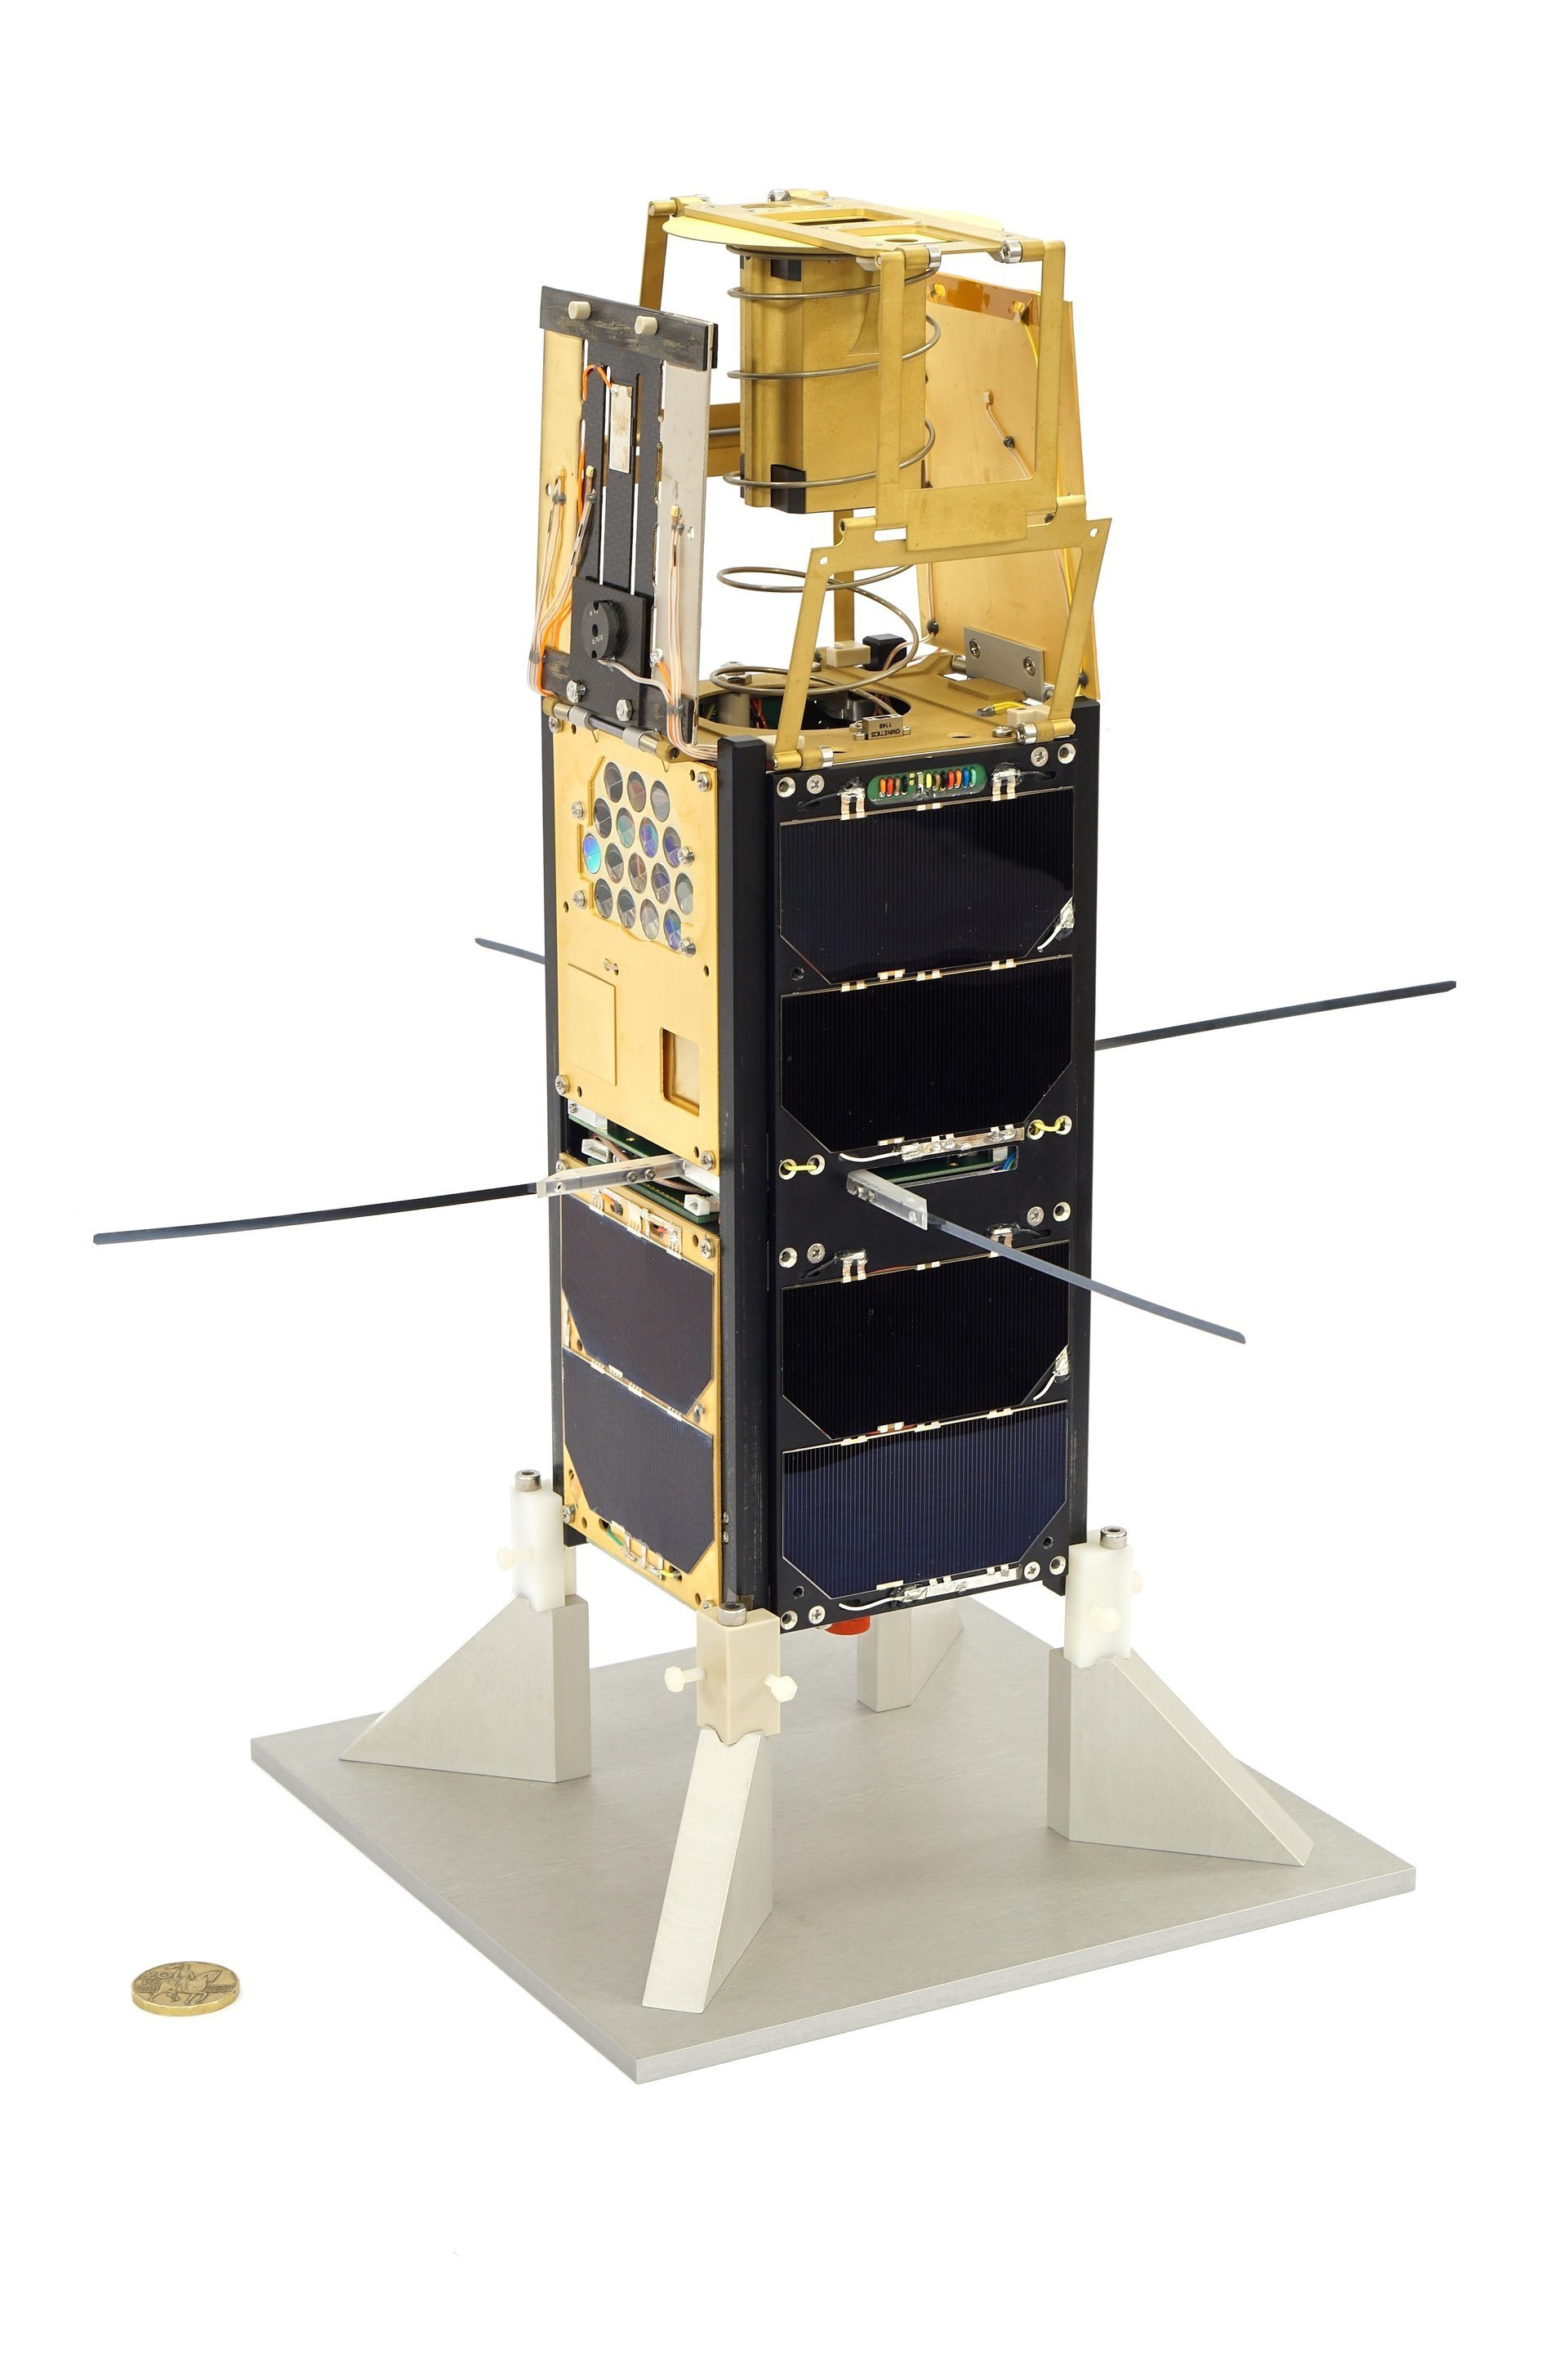
\includegraphics[height=0.9\textheight]{./fig/photos/vzlusat_whole2.jpg}

\end{columns}

\end{frame}

\begin{frame}
\frametitle{VZLUSAT-1 --- Space weather dosimetry (2018--2021)}

\vspace{-0.5em}

\begin{columns}[c]

\column{0.48\textwidth} % Left column and width
\includegraphics[width=1.0\textwidth,trim={1cm 3.0cm 0cm 3.5cm},clip]{./fig/plots/vzlusat_map.eps}

\column{0.48\textwidth} % Right column and width
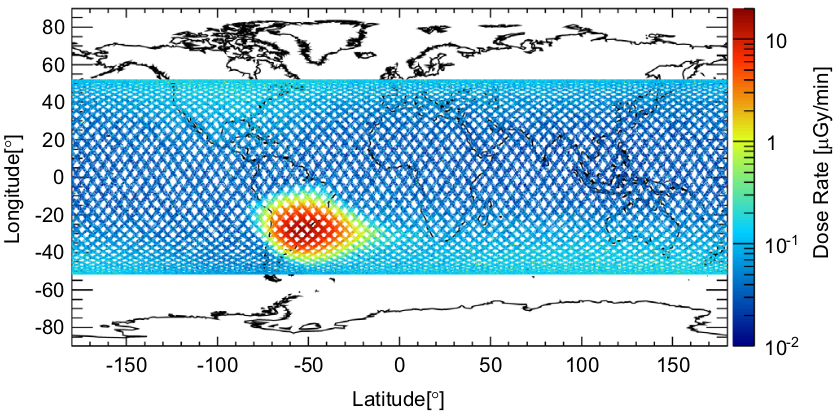
\includegraphics[width=1.0\textwidth,trim={0cm 1.0cm 0cm 0.0cm},clip]{./fig/plots/iss_map_2.png}

\end{columns}

\vspace{-1em}

\begin{center}
  Ionizing radiation dose measured by the Timepix sensor onboard (left) VZLUSAT-1 ($\approx 500$\,km Sun-synchronous orbit), and (right) the ISS ($\approx 350$\,km orbit).
\end{center}

\vspace{-0.5em}

\begin{block}{Data publicly available}
  \centering
  \url{https://github.com/vzlusat/vzlusat1-timepix-data}
\end{block}

\vspace{-0.5em}

\fullciteinbox{baca2018timepix}{}

\end{frame}

%%}

%%{ REX

\begin{frame}
\frametitle{REX --- Rocket Experiment}

\begin{columns}[c]

\column{0.65\textwidth} % Left column and width

\begin{block}{NASA's Sounding Rocket launch (2018) \cite{urban2021rex}}
  \begin{itemize}
    \item Collaboration with PennState university (PA, USA)
    \item 2 X-Ray telescopes, 2 Timepix detectors
    \item ROS-powered onboard computers with Rospix \cite{baca2018rospix}
  \end{itemize}
\end{block}

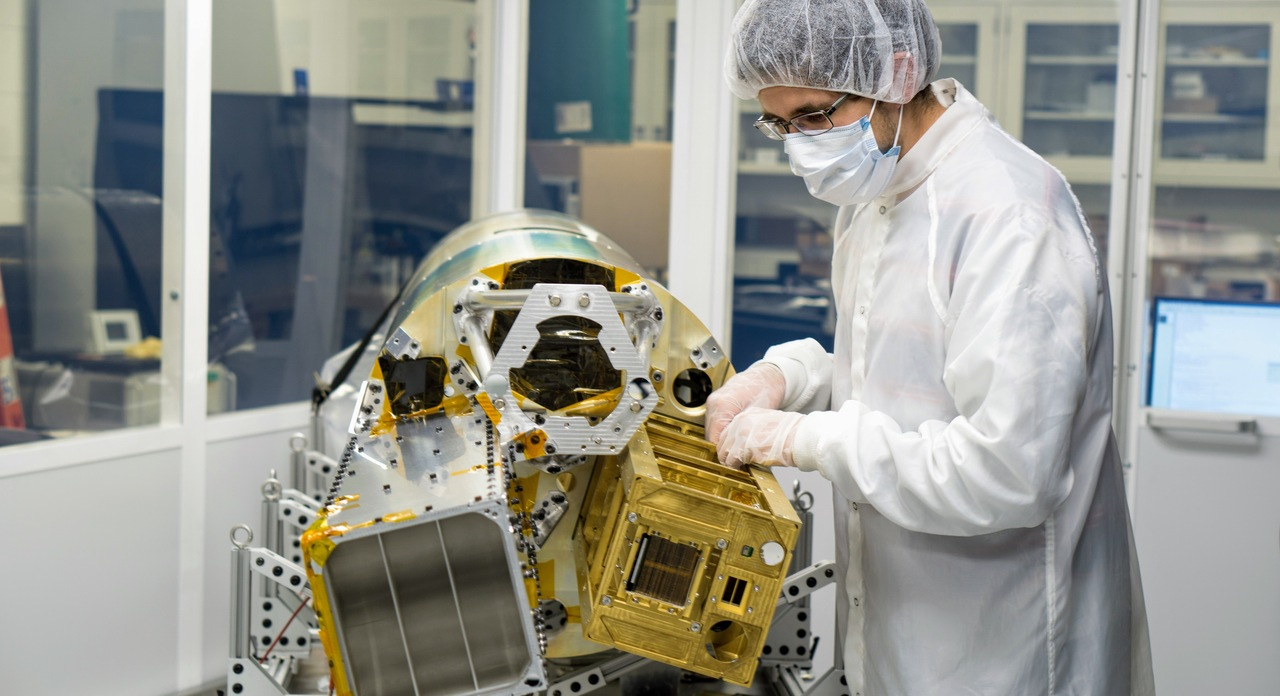
\includegraphics[width=0.9\textwidth]{./fig/photos/rocket_tomas.jpg}

\column{0.3\textwidth} % Right column and width

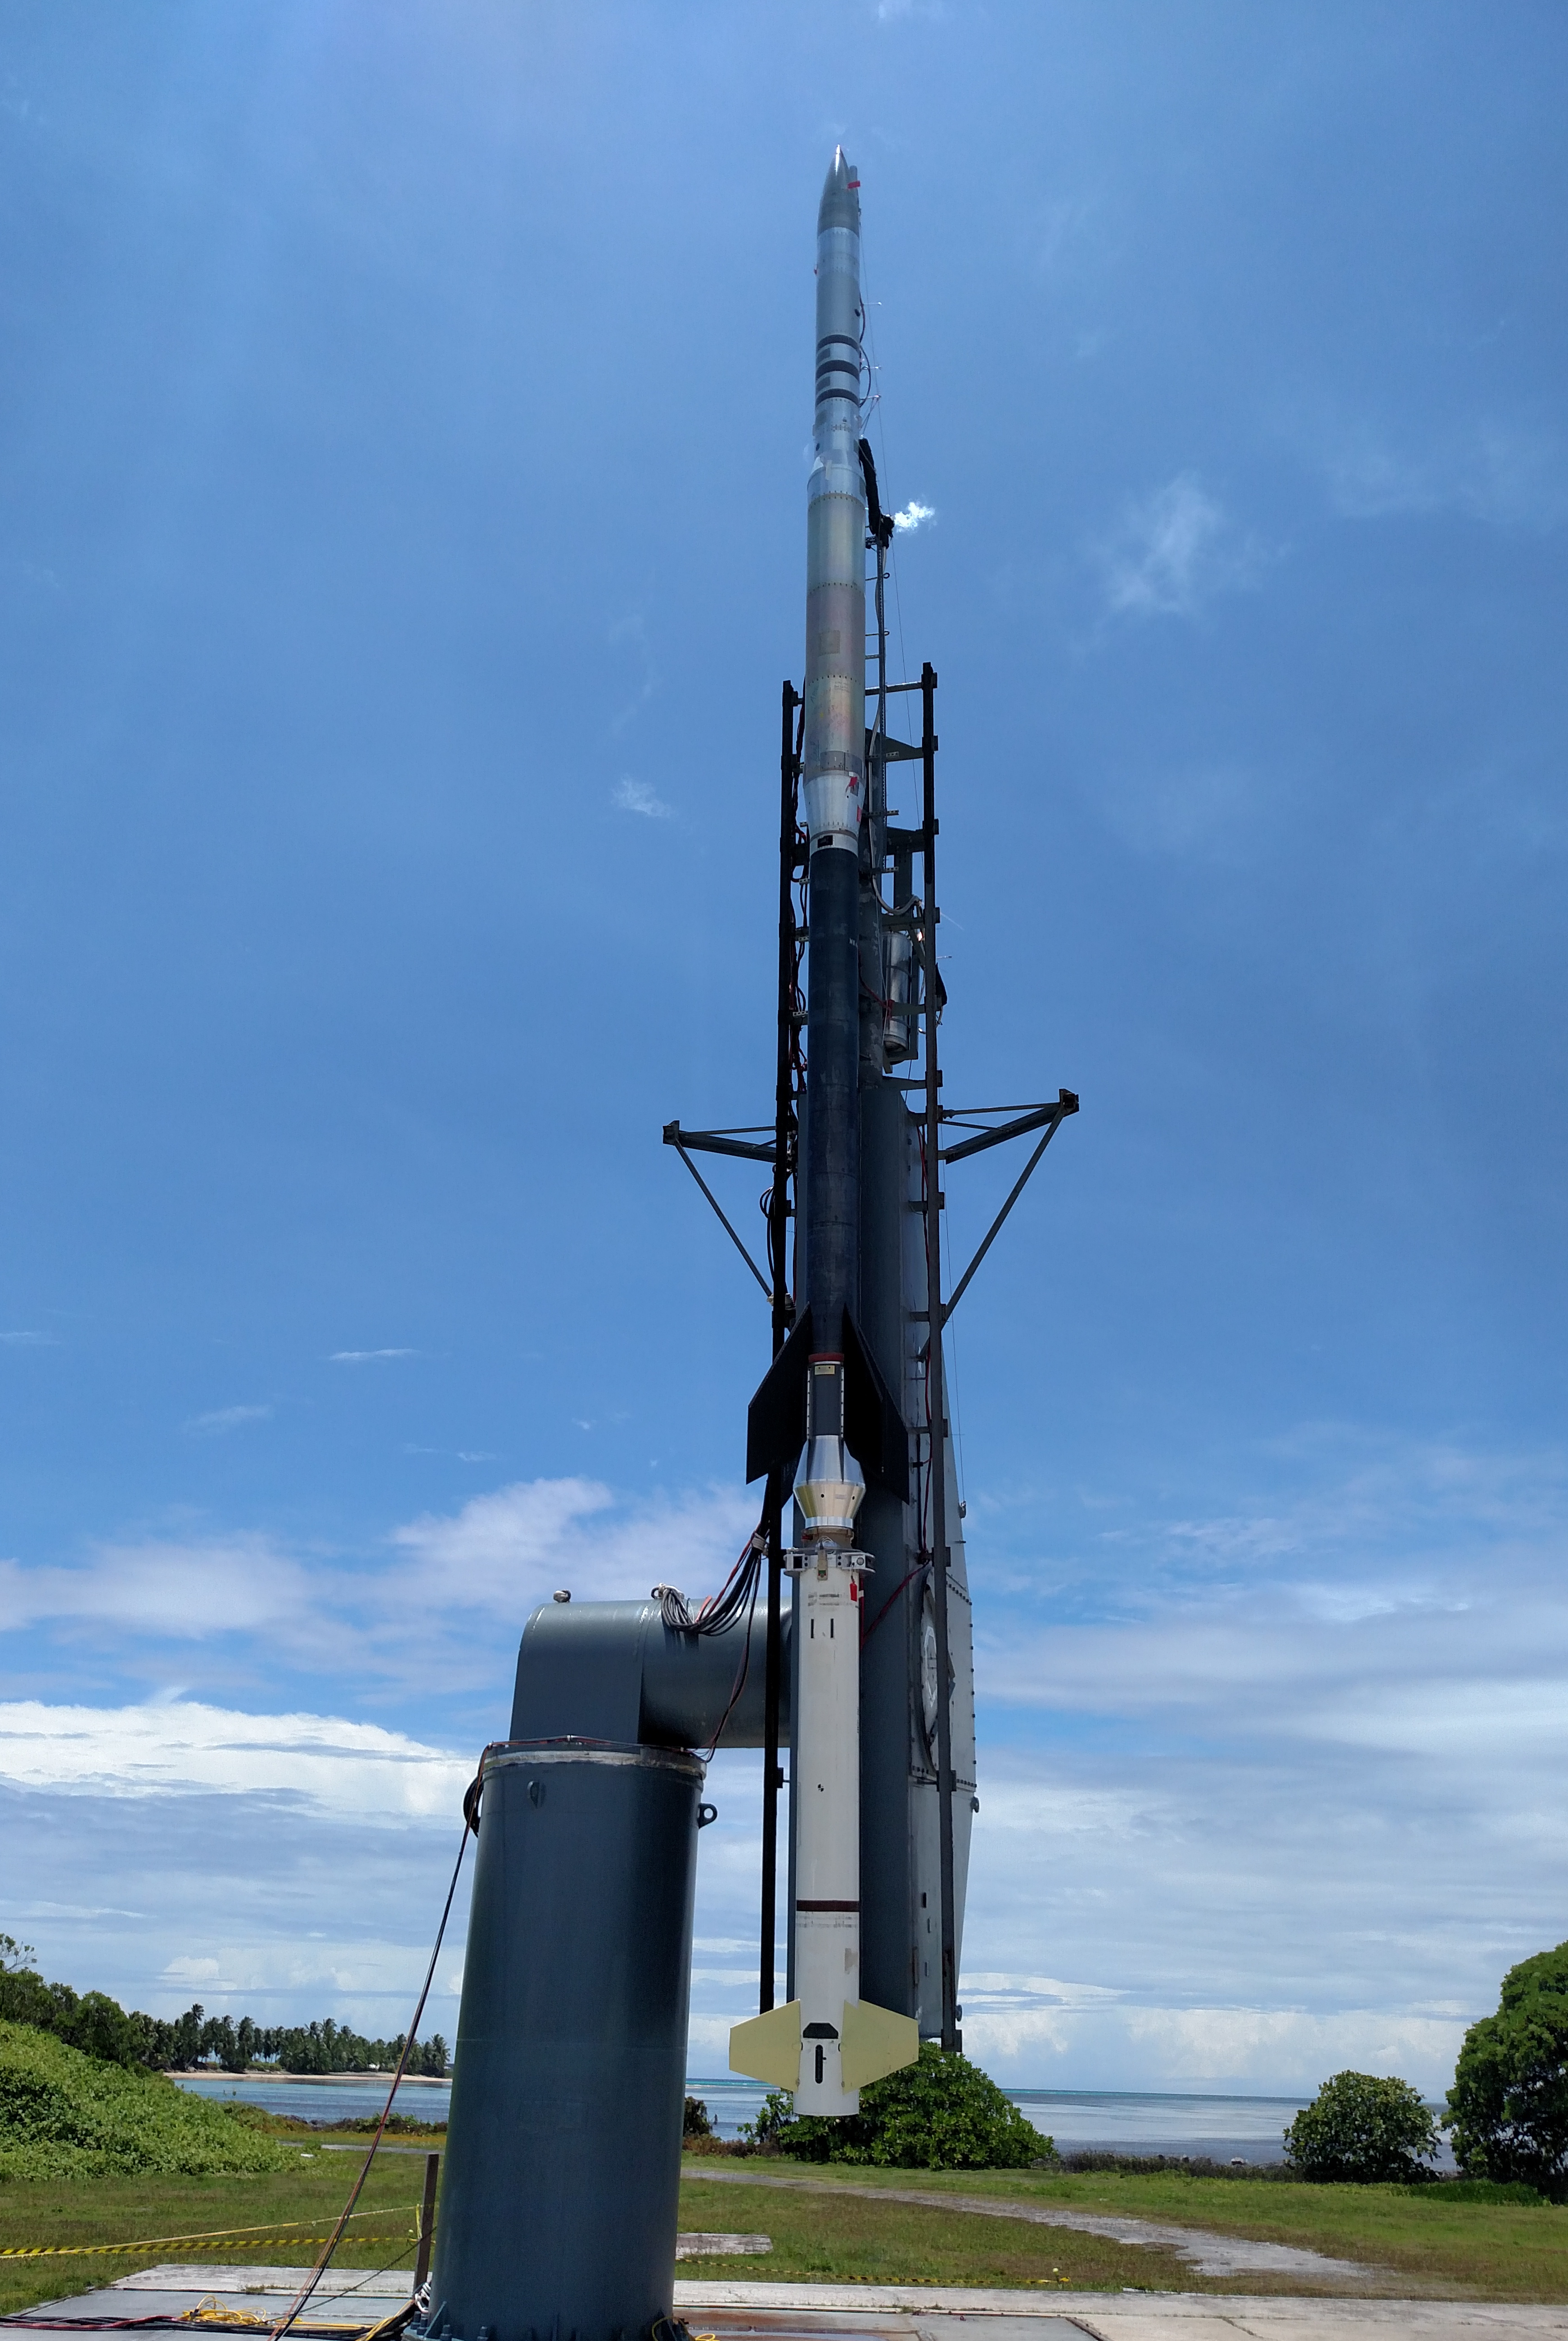
\includegraphics[height=0.85\textheight]{./fig/photos/rocket.jpg}

\end{columns}

\end{frame}

%%}

%%{ Timepix onboard UAVs

\begin{frame}
\frametitle{Timepix detector onboard UAVs}

\begin{block}{Proof of concept for UAVs}
  \begin{itemize}
    \item real-time ray-tracing Timepix simulation model
    \item real-time particle track classifier
    \item verification of the simulation model vs. reality
  \end{itemize}
\end{block}

\begin{figure}
  \begin{adjustbox}{max totalsize={1.0\textwidth}, center}
    \pgfdeclarelayer{foreground}
\pgfsetlayers{background,main,foreground}

\tikzset{radiation/.style={{decorate,decoration={expanding waves,angle=90,segment length=4pt}}}}

\begin{tikzpicture}[->,>=stealth', node distance=3.1cm]

  \node[state, shift = {(0.0, 0.0)}] (timepix) {
      \begin{tabular}{c}
        \small Timepix\\
        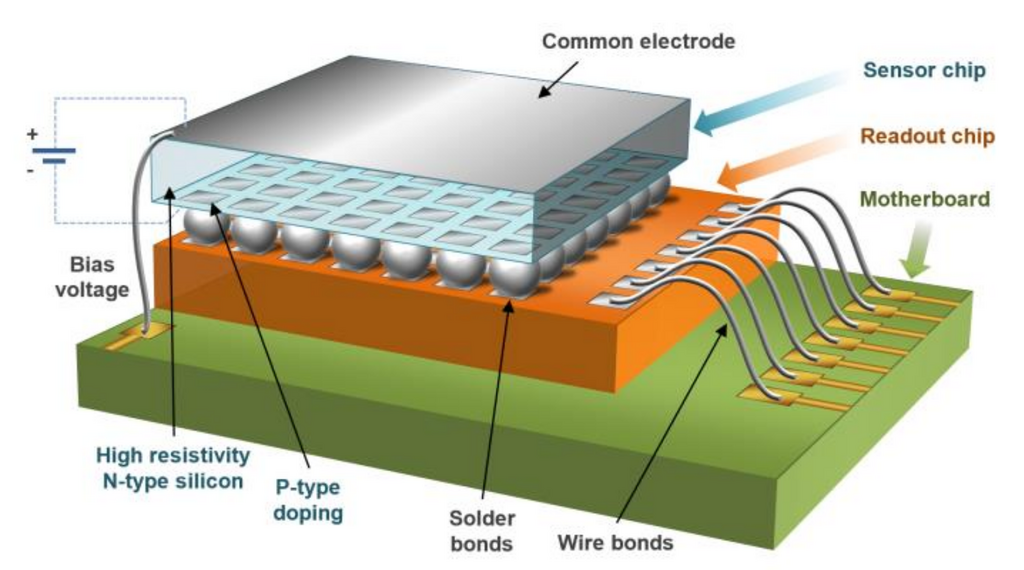
\includegraphics[width=1.7cm]{./fig/photos/timepix_structure.png}
      \end{tabular}
    };

  \node[state, right of = timepix, shift = {(-0.25, 0.0)}] (readout) {
      \begin{tabular}{c}
        \small USB interface\\
        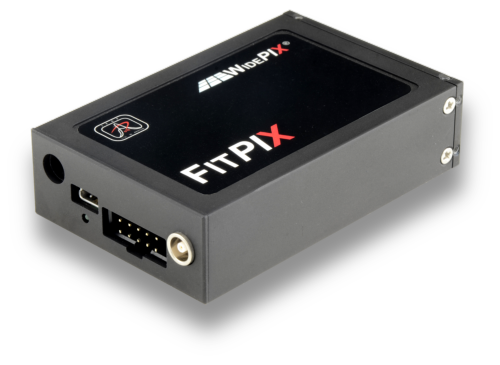
\includegraphics[width=1.7cm]{./fig/photos/fitpix_small.png}
      \end{tabular}
    };

  \node[state, right of = readout, shift = {(-0.20, -0)}] (rospix) {
      \begin{tabular}{c}
        \small Rospix\\
        \frame{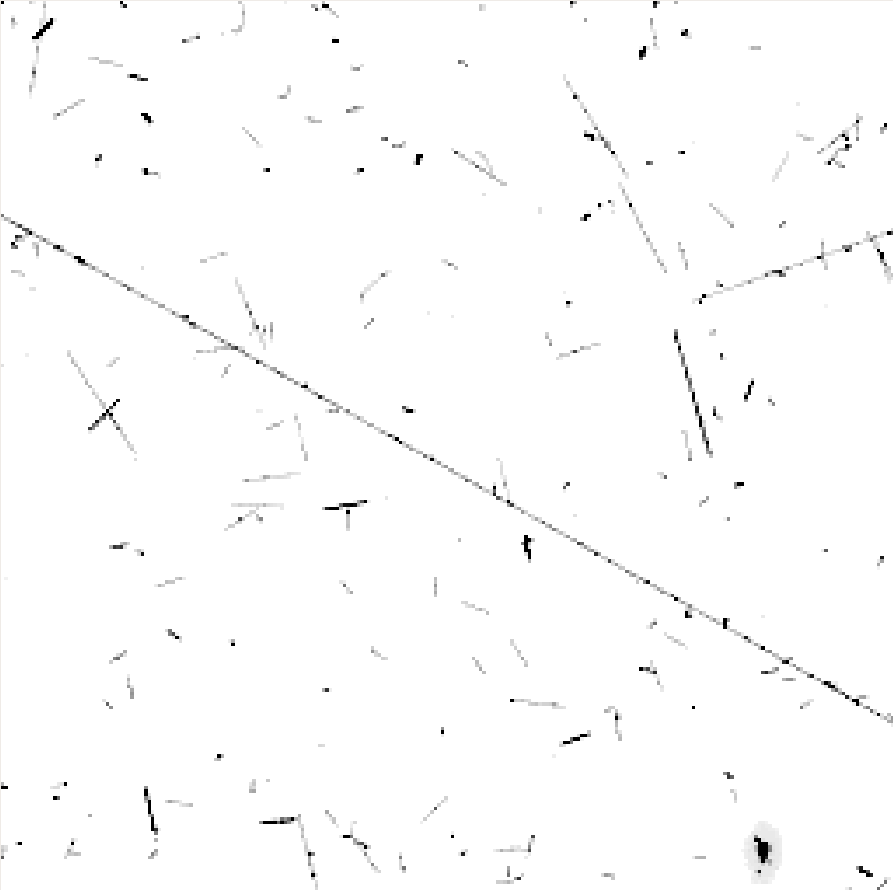
\includegraphics[width=1.7cm]{./fig/photos/image_4.png}}
      \end{tabular}
    };

  \node[state, right of = rospix, shift = {(0.2, -0)}] (track_classification) {
      \begin{tabular}{c}
        \small Track classification\\
        \frame{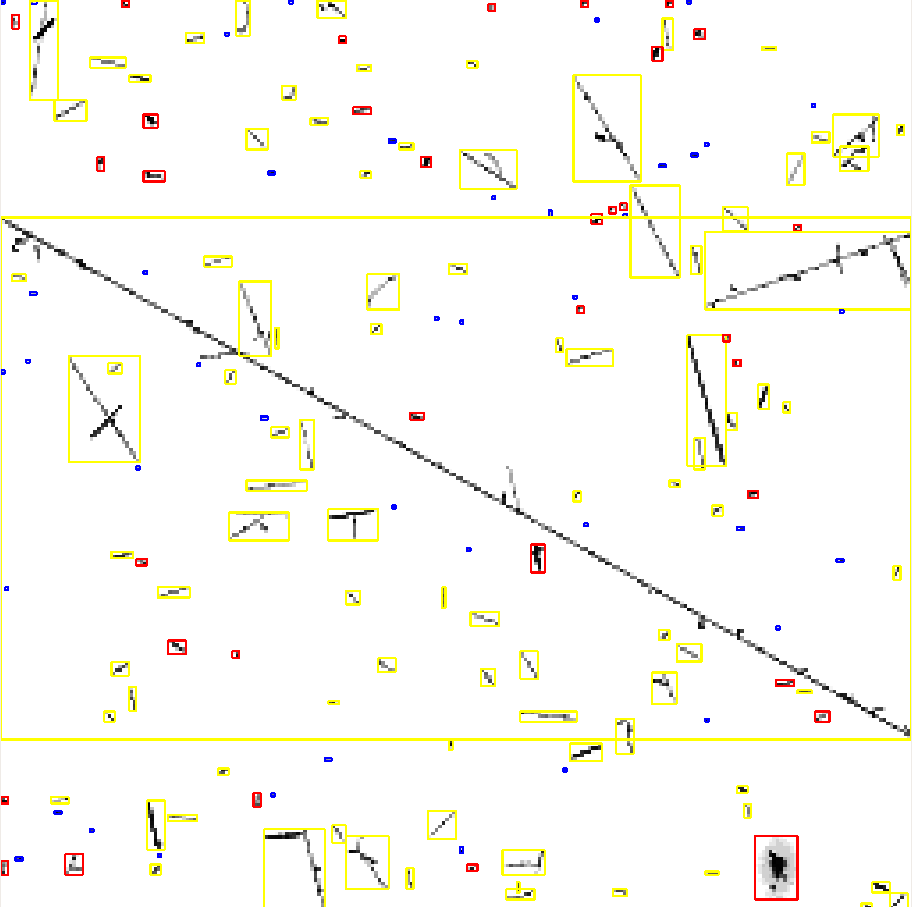
\includegraphics[width=1.7cm]{./fig/photos/classified_image_4.png}}
      \end{tabular}
    };

  \node[state, right of = track_classification, shift = {(0.6, -0)}] (estimation) {
      \begin{tabular}{c}
        \small Target estimation\\
        \frame{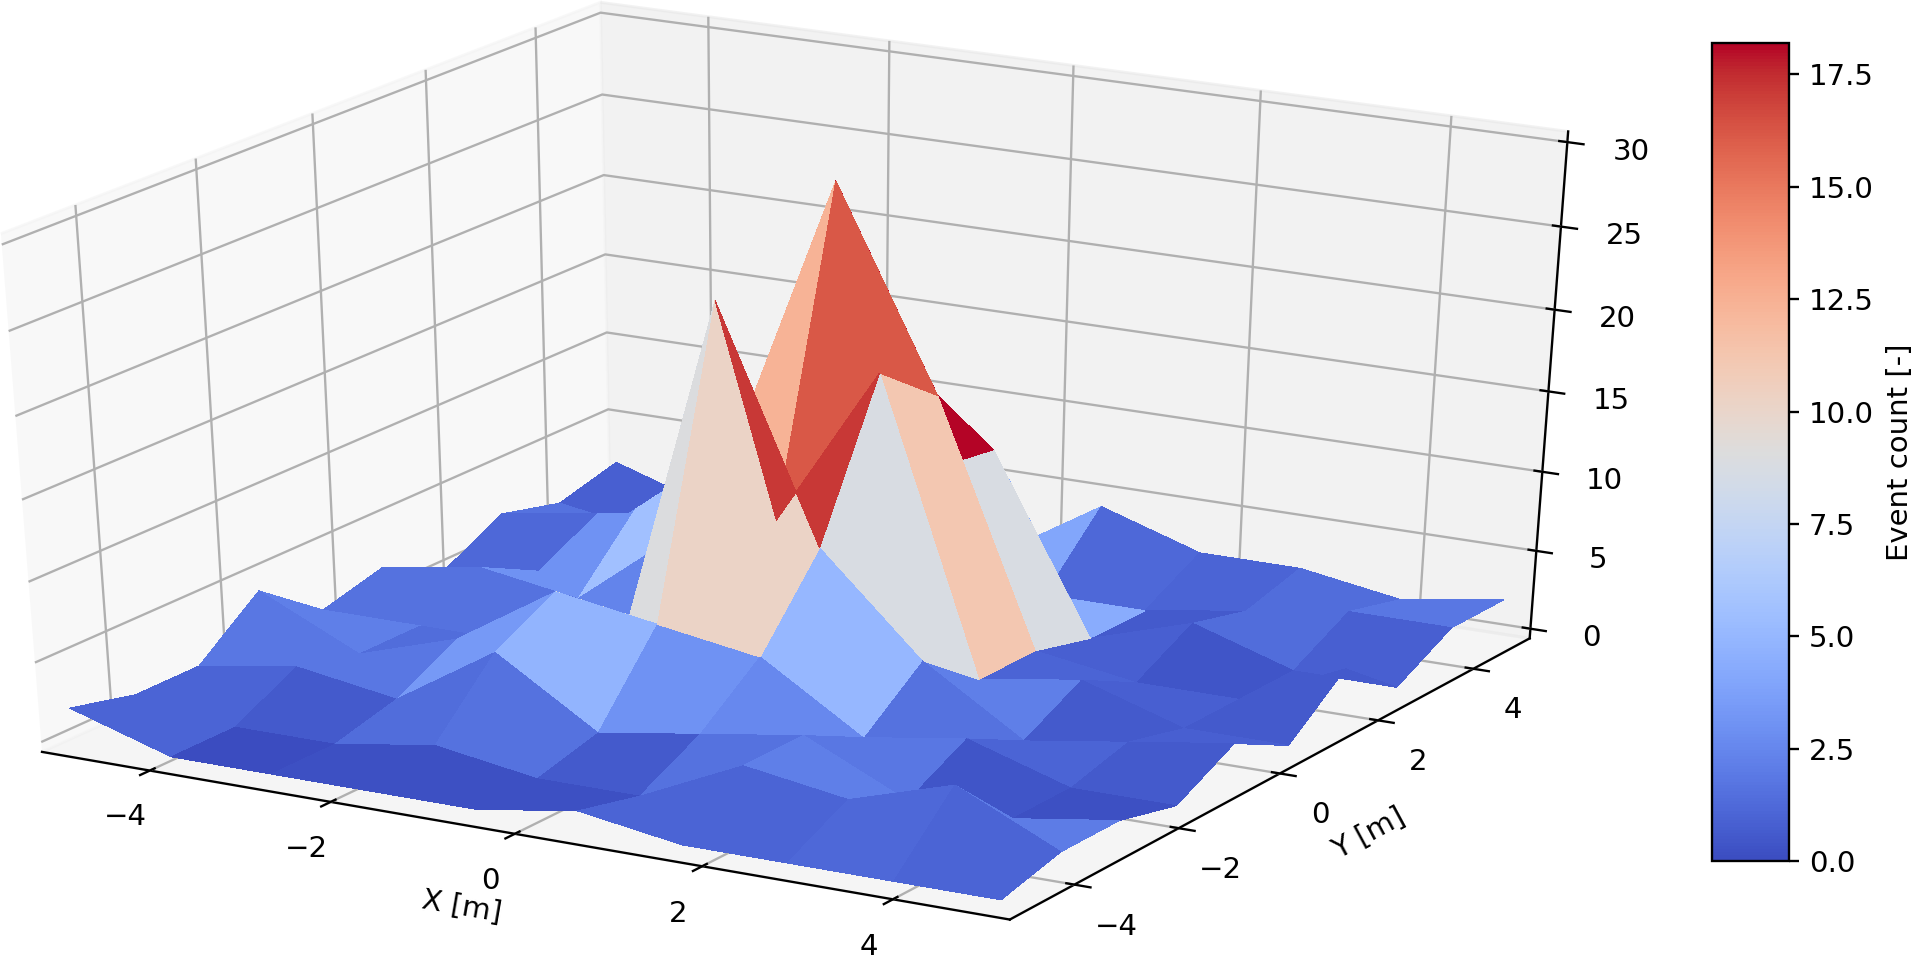
\includegraphics[width=1.7cm]{./fig/photos/Photons.png}}
      \end{tabular}
    };

  \node[state, right of = estimation, shift = {(-0.2, -0)}] (feedback) {
      \begin{tabular}{c}
        UAV\\feedback\\control
      \end{tabular}
    };

  \path[->] ($(timepix.east) + (0.0, 0)$) edge [] node[above, midway, shift = {(0.0, 0.05)}] {
      \begin{tabular}{c}
    \end{tabular}} ($(readout.west) + (0.0, 0.00)$);

  \path[->] ($(readout.east) + (0.0, 0)$) edge [] node[above, midway, shift = {(0.0, 0.05)}] {
      \begin{tabular}{c}
    \end{tabular}} ($(rospix.west) + (0.0, 0.00)$);

    \path[->] ($(rospix.east) + (0.0, 0)$) edge [] node[above, midway, shift = {(0.0, 0.05)}] {
      \begin{tabular}{c}
    \end{tabular}} ($(track_classification.west) + (0.0, 0.00)$);

    \path[->] ($(track_classification.east) + (0.0, 0)$) edge [] node[above, midway, shift = {(0.0, 0.05)}] {
      \begin{tabular}{c}
    \end{tabular}} ($(estimation.west) + (0.0, 0.00)$);

    \path[->] ($(estimation.east) + (0.0, 0)$) edge [] node[above, midway, shift = {(0.0, 0.05)}] {
      \begin{tabular}{c}
    \end{tabular}} ($(feedback.west) + (0.0, 0.00)$);

    \pgfmathsetmacro{\offsetA}{0.2}
    \coordinate (above_rospix) at ($(rospix.north) + (0.0, \offsetA)$);
    \coordinate (above_classification) at ($(track_classification.north) + (0.0, \offsetA)$);
    \path[-] ($(track_classification.north) + (0.0, 0)$) edge [] (above_classification) -- (above_classification) edge [] (above_rospix) edge [] node[midway, shift = {(0.0, 0.20)}] {  
      \begin{tabular}{c}
        \small acquisition control
    \end{tabular}} (above_rospix) -- (above_rospix) edge [->] ($(rospix.north) + (0.0, 0.0)$);

    % \path[->] ($(timepix.east) + (0.15, 1.0)$) edge [dotted] node[above, near start, shift = {(0.0, 0.15)}] {
    %   \begin{tabular}{c}
    %     LVDS
    % \end{tabular}} ($(timepix.east) + (0.15, 0.0)$);

    % \path[->] ($(readout.east) + (0.15, 1.4)$) edge [dotted] node[above, near start, shift = {(0.0, 0.30)}] {
    %   \begin{tabular}{c}
    %     USB
    % \end{tabular}} ($(readout.east) + (0.15, 0.0)$);

    % \begin{pgfonlayer}{background}
    %   \path (rospix.west |- rospix.north)+(-0.20, 0.60) node (a) {};
    %   \path (track_classification.south -| track_classification.east)+(0.20,-0.5) node (b) {};
    %   \path[fill=gray!0, draw=black!50, dashed]
    %   (a) rectangle (b);
    %   \path (rospix.west |- rospix.south)+(-0.20, 0.0) -- node [midway, shift = {(0.0, -0.3)}] {\begin{tabular}{c}
    %       \small Proposed ROS pipeline
    %   \end{tabular}} (track_classification.south -| track_classification.east);
    % \end{pgfonlayer}

  \end{tikzpicture}

  \end{adjustbox}
\end{figure}

\fullciteinbox{baca2019timepix}{}

\end{frame}

%%}

\begin{frame}
\frametitle{Ionizing radiation dosimetry and imaging}

\begin{columns}[c]

\column{0.65\textwidth} % Left column and width
\begin{block}{UAV Experiment in SUJCHBO}
  \begin{center}
    \mymovie[autostart,loop,start=100]{
      \includegraphics[width=0.90\textwidth]{./videos/rospix_uav_flight_thumbnail.jpg}
    }{./videos/rospix_uav_flight.mp4}\\
  \end{center}
\end{block}

\column{0.30\textwidth} % Right column and width

\begin{itemize}
  \item \isotope[241]{Am}, $\approx$ \SI{500}{\mega\Bq}
  \item Timepix, Si \SI{300}{\micro\meter}
  \item FITPix readout
\end{itemize}

\end{columns}

\end{frame}

\begin{frame}
\frametitle{Ionizing radiation dosimetry and imaging}

\begin{block}{Multi-UAV source estimation}
  \begin{itemize}
    \item exploiting measurement directionality
    \item environment with obstacles
    \item UAVs change heading to estimate bearing
    \item scalable Multi-UAV source estimation
    \item verified in Gazebo simulations
  \end{itemize}
\end{block}

\fullciteinbox{stibinger2020localization}{}

\end{frame}

%%}

%%{ Publication record

\begin{frame}
\frametitle{Publication record}

\begin{columns}[c]

\column{0.48\textwidth} % Left column and width

\begin{block}{Publications during Ph.D}
  \begin{itemize}
    \item \makebox[2.2cm]{Total:\hfill} 45
    \item \makebox[2.2cm]{Imp. Journal:\hfill} 28
    \item \makebox[2.2cm]{Conference:\hfill} 17
    \item \makebox[2.2cm]{First author:\hfill} 11
  \end{itemize}
\end{block}

  \begin{block}{Top-cited publications ($1^{\text{st}}$ author)}
  \begin{itemize}
    \item \makebox[2.2cm]{\cite{baca2016miniaturized}:\hfill} 16
    \item \makebox[2.2cm]{\cite{baca2018model}:\hfill} 7
    \item \makebox[2.2cm]{\cite{baca2017autonomous}:\hfill} 7
    \item \makebox[2.2cm]{\cite{baca2019autonomous}:\hfill} 6
  \end{itemize}
\end{block}

\column{0.48\textwidth} % Right column and width

\begin{block}{Citations}
  \begin{itemize}
    \item \makebox[2.7cm]{WoS no autocit:\hfill} 194
    \item \makebox[2.7cm]{WoS all:\hfill} 319
    \item \makebox[2.7cm]{Scopus:\hfill} 517
    \item \makebox[2.7cm]{Google scholar:\hfill} 1198
  \end{itemize}
\end{block}

\begin{block}{H-index}
  \begin{itemize}
    \item \makebox[2.7cm]{WoS no autocit:\hfill} 8
    \item \makebox[2.7cm]{WoS all:\hfill} 11
    \item \makebox[2.7cm]{Scopus:\hfill} 12
    \item \makebox[2.7cm]{Google scholar:\hfill} 18
  \end{itemize} 
\end{block}

\end{columns}

\end{frame}

%%}

%%{ Projects

\begin{frame}
\frametitle{Projects}

\begin{block}{TACR RADRON (2020-2022), FW0101317, $8^{\mathrm{th}}$ of 396 submitted}
  \begin{itemize}
    \item \textbf{Source}: Technology Agency of the Czech Republic , $\approx$ \$1M USD
    \item \textbf{Title}: \emph{Localization of sources of ionizing radiation using a group of small unmanned aircrafts with Compton camera detectors}
    \item \textbf{PI}: \emph{Advacam, s.r.o.}, \textbf{Co-I}: Czech metrology institute
    \item \textbf{Contribution}: Devised the estimation methodology, co-wrote the project with the PI
  \end{itemize}
\end{block}

\begin{block}{TACR Glamr (2021-2023), FW03010020, $13^{\mathrm{th}}$ of 433 submitted}
  \begin{itemize}
    \item \textbf{Source}: Technology Agency of the Czech Republic , $\approx$ \$2.2M USD
    \item \textbf{Title}: \emph{Guidance and Localization upgrade creating Autonomous Mobile Robots}
    \item \textbf{PI}: \emph{DataVision, s.r.o.}
    \item \textbf{Contribution}: Devised the UAV methodology, co-wrote the project with the PI
  \end{itemize}
\end{block}

\end{frame}

%%}

%%{ Publication graph

\begin{frame}
\frametitle{Research streams}

\begin{columns}[c]

\column{0.48\textwidth} % Left column and width

\centering

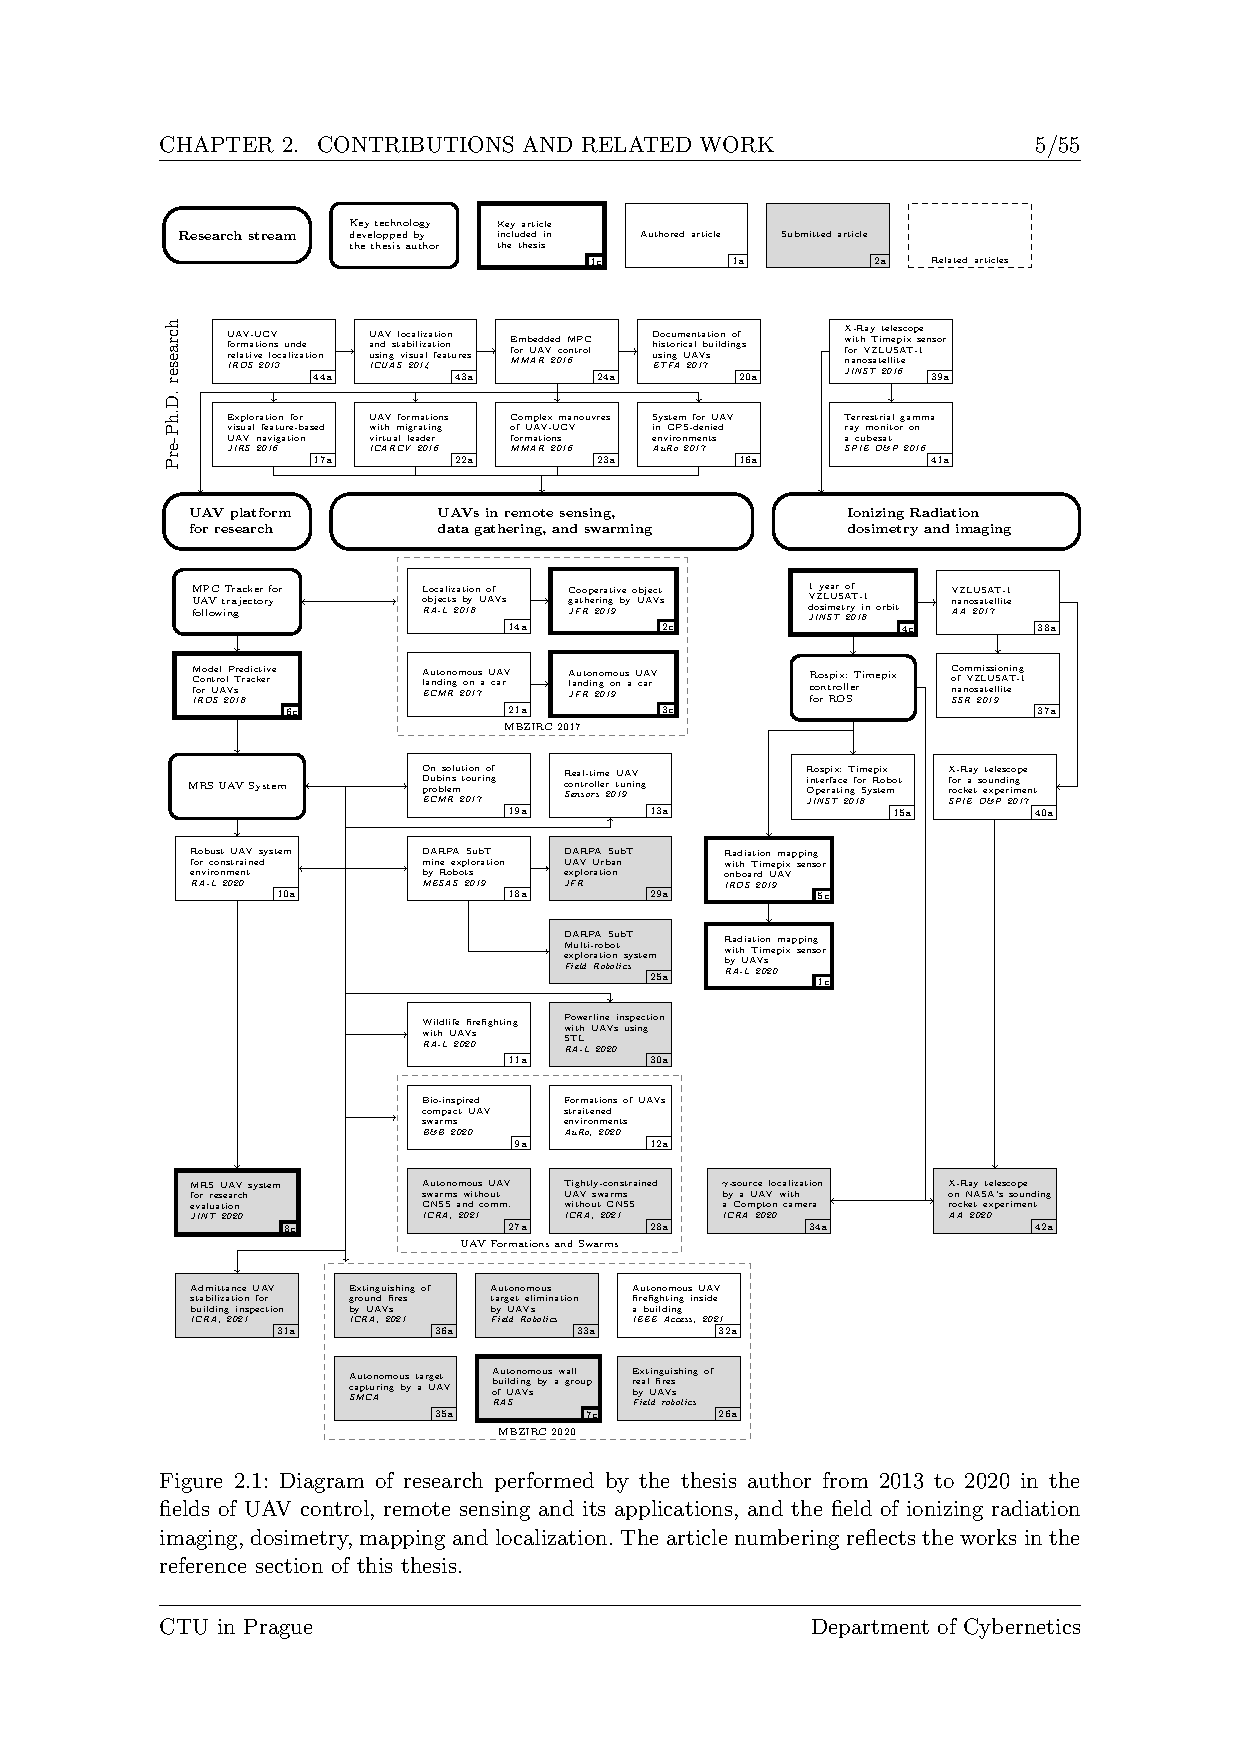
\includegraphics[width=0.9\textwidth,trim={2.0cm 5.0cm 2.5cm 5.2cm},clip]{./fig/pubgraph_january.pdf}

\centering

\column{0.48\textwidth} % Right column and width

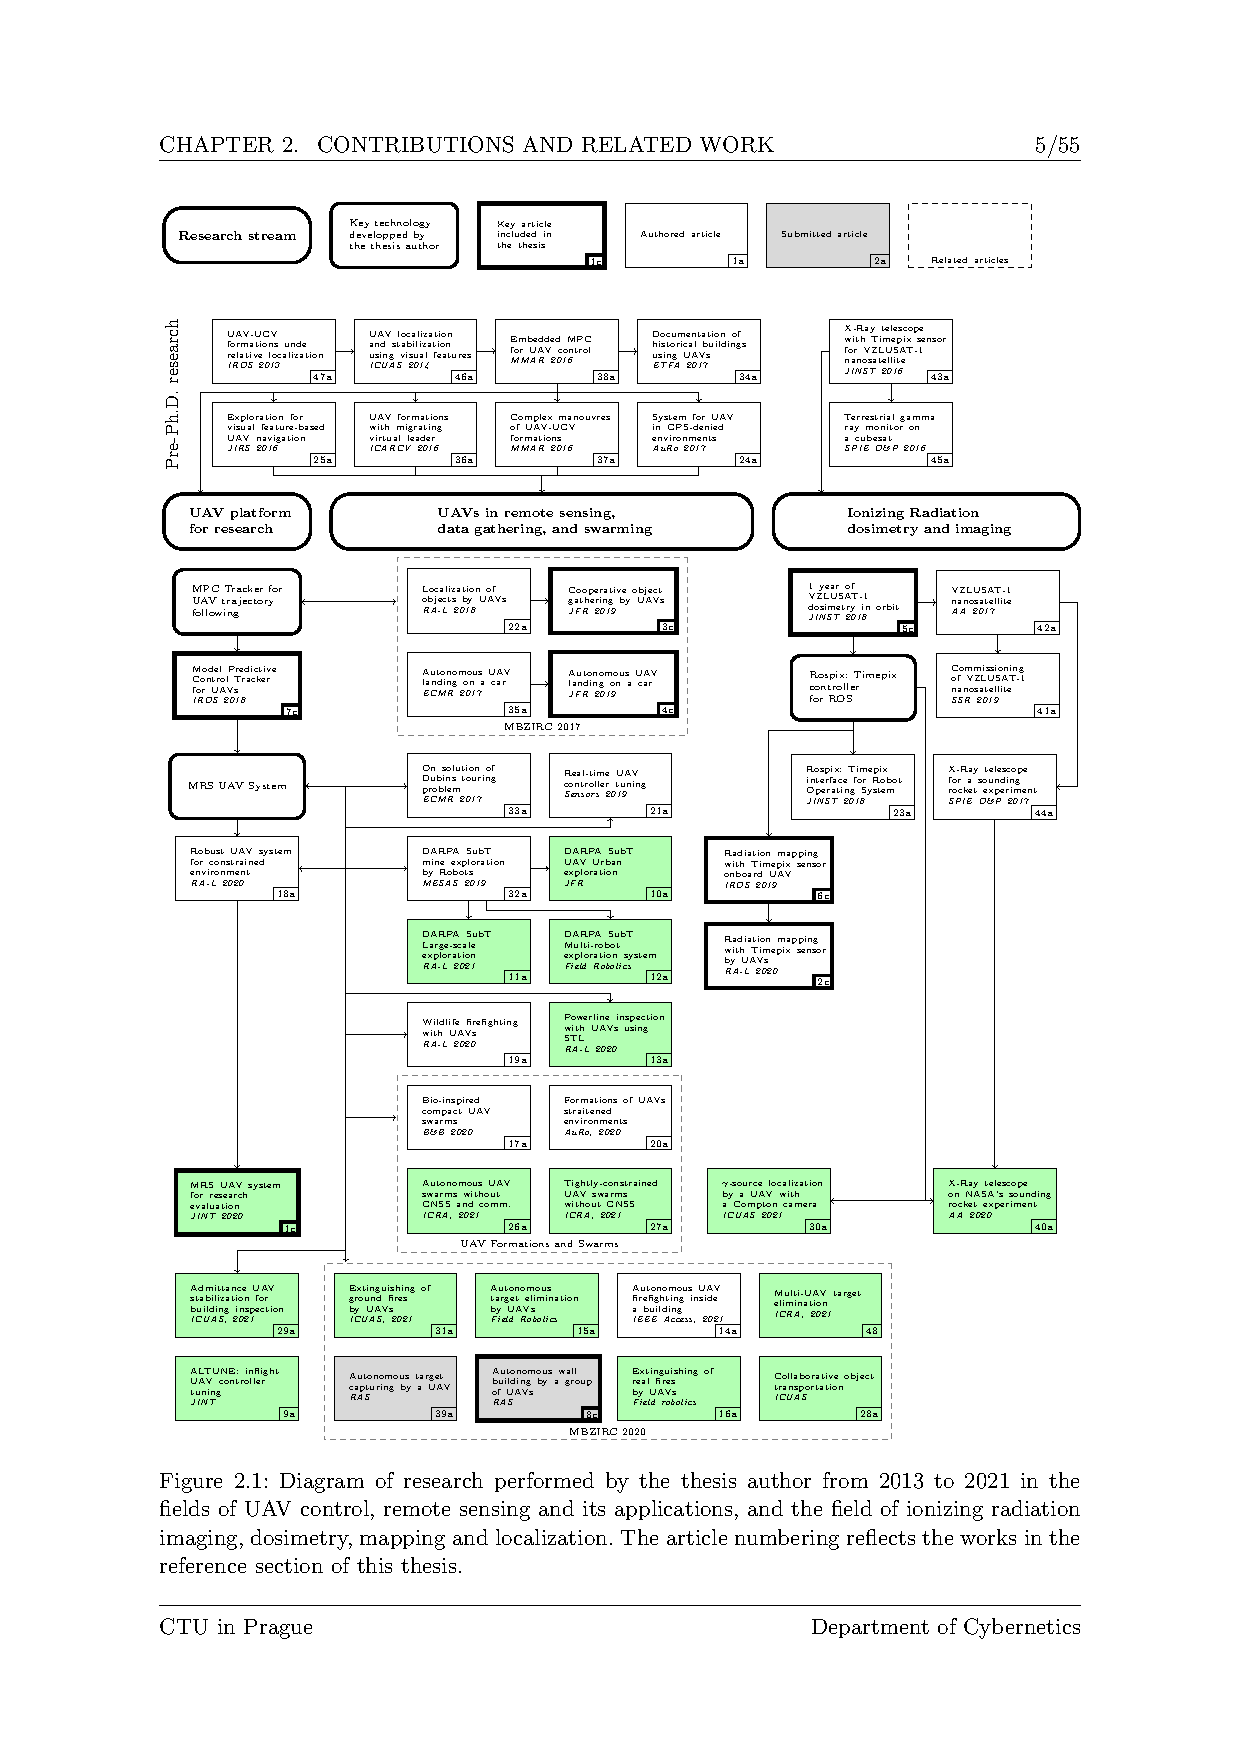
\includegraphics[width=0.9\textwidth,trim={2.0cm 5.0cm 2.5cm 5.2cm},clip]{./fig/pubgraph.pdf}

\end{columns}

\end{frame}

%%}

\begin{frame}
\frametitle{The MRS Team}

  \begin{columns}[c]
  
  \column{0.48\textwidth} % Left column and width

  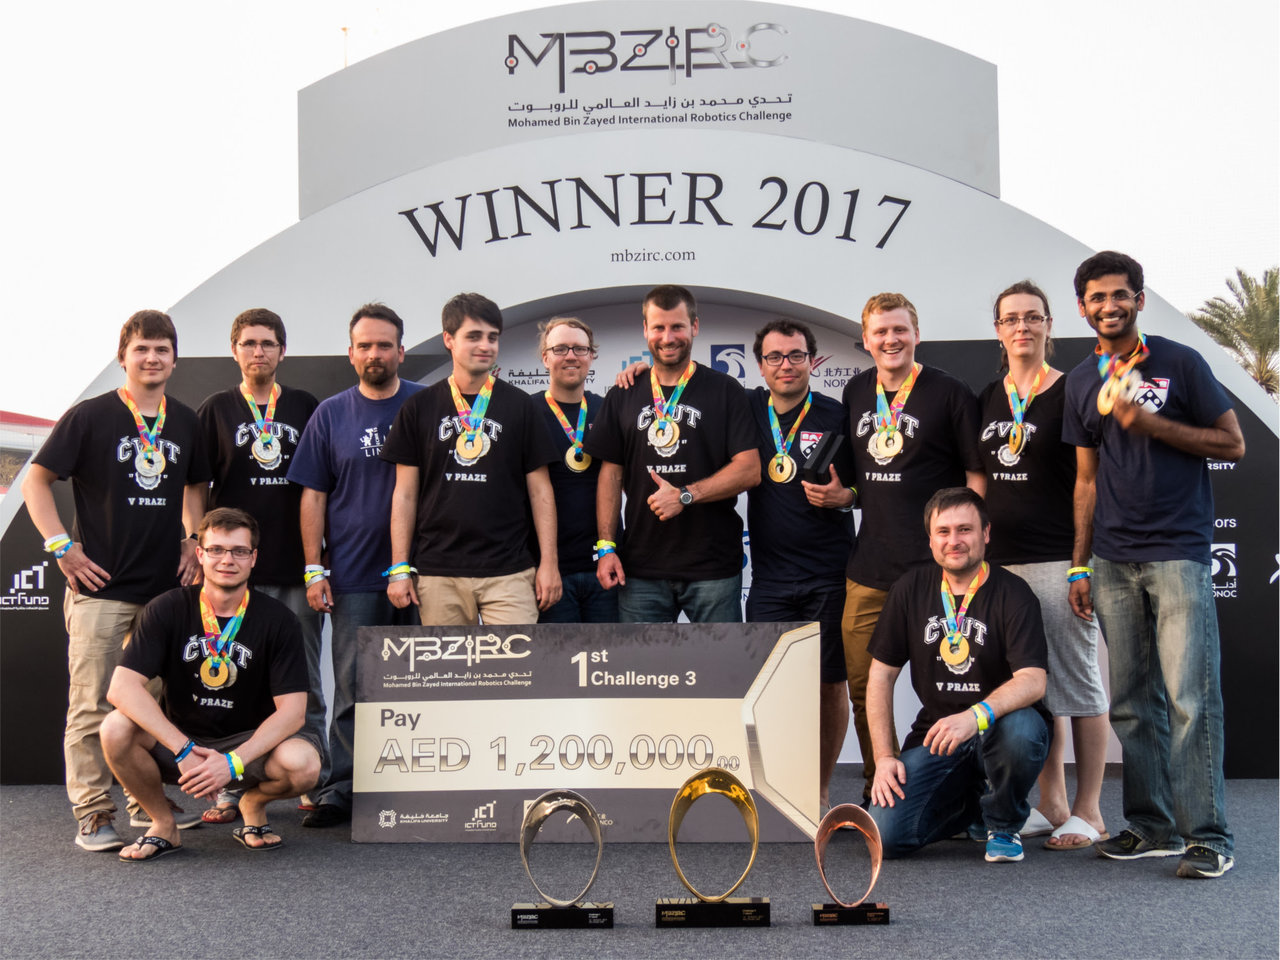
\includegraphics[width=1.0\textwidth]{./fig/photos/mbzirc_team_2017.jpg}
  
  \column{0.48\textwidth} % Right column and width
  
  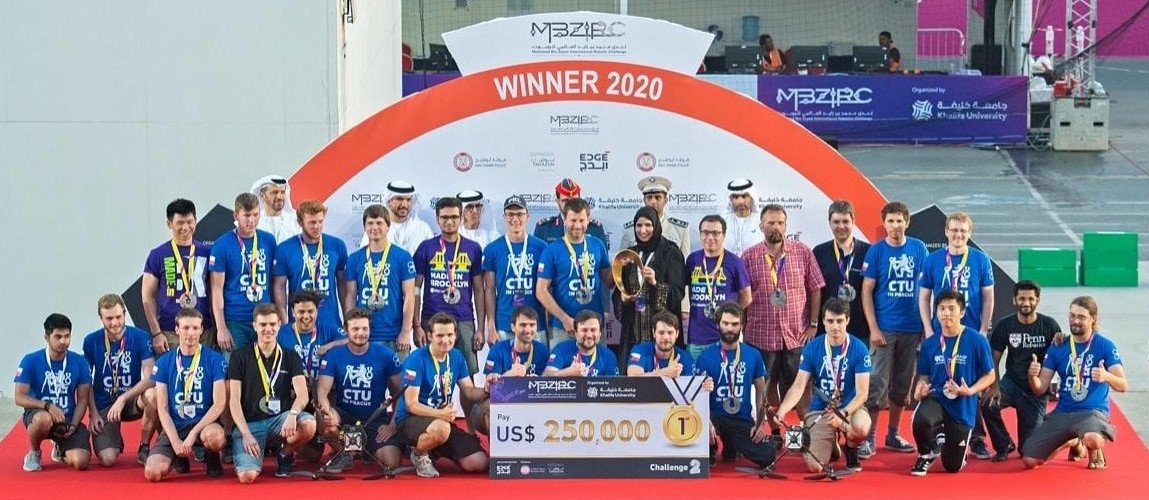
\includegraphics[width=1.0\textwidth]{./fig/photos/mbzirc_team_2020.jpg}
  
  \end{columns}

\end{frame}

\section{Discussion and results}

%%{ Discussion 

\begin{frame}
\frametitle{Discussion and results}

\end{frame}

%%}

%%{ Conclusion

\begin{frame}
  \frametitle{Conclusion}

  \begin{center}
    \huge Thanks for your attention\\
    \vspace{1em}
    \large \url{http://mrs.felk.cvut.cz/people/tomas-baca}
  \end{center}

\end{frame}

%%}

%%{ References

\DeclareCiteCommand{\fullcite}
{\usebibmacro{prenote}}
{\clearfield{addendum}%
  \usedriver
  {\defcounter{minnames}{6}%
  \defcounter{maxnames}{6}}
{\thefield{entrytype}}}
{\multicitedelim}
{\usebibmacro{postnote}}

\begin{frame}
  \frametitle{Core publications}
  \tiny{
    \printbibliography[keyword={mine},keyword={phd_related},keyword={core},heading=none,title={}]
  }
\end{frame}

\begin{frame}[allowframebreaks]
  \frametitle{Other authored publications}
  \tiny{
    \printbibliography[keyword={mine},notkeyword={core},heading=none,title={}]
  }
\end{frame}

%%}

%% | ---------------------- BACKUP SLIDES --------------------- |

%%{ Research visits and stays

\begin{frame}[noframenumbering]
\frametitle{Research visits and stays abroad}

  \begin{itemize}
    \item 2015 University of Iowa, USA, 2 weeks, \emph{X-Ray testing of VZLUSAT-1 payload}
    \item 2016 University of Pennsylvania, USA, 2 months, \emph{kick-off for MBZIRC 2017}
    \item 2017 United Arab Emirates, 3 weeks, \emph{MBZIRC 2017}
    \item 2017 Pennsylvania state Univ., USA, 2 weeks, \emph{REX X-Ray testing}
    \item 2018 University of Pennsylvania, USA, 1 month, \emph{kick-off for MBZIRC 2020}
    \item 2018 Pennsylvania state Univ., USA, 2 weeks, \emph{REX assembly}
    \item 2019 Colorado, USA, 2 weeks, \emph{DARPA SubT STIX}
    \item 2019 Pennsylvania state Univ., USA, 1 week, \emph{REX dissassembly}
    \item 2020 United Arab Emirates, 5 weeks, \emph{MBZIRC 2020}
    \item 2021 United Arab Emirates, 1 month, \emph{TII collaboration}
    \item 2021 Kentucky, USA, 3 weeks, \emph{DARPA SubT Finals}
  \end{itemize}

\end{frame}

%%}

\end{document}
